\documentclass[11pt,a4paper]{article}
\usepackage[utf8]{inputenc}
\usepackage[T1]{fontenc}
\usepackage{lmodern}
\usepackage[margin=25mm]{geometry}
\usepackage{amsmath,amssymb,mathtools,bm,array,xcolor,booktabs,longtable}
\usepackage{tikz,microtype,enumitem}
\usepackage[nolist]{acronym}
\usetikzlibrary{arrows.meta,positioning,fit}
\usepackage[colorlinks=true,linkcolor=blue!50!black,urlcolor=blue!50!black]{hyperref}
\newenvironment{example}[1]{\par\medskip\noindent\textbf{Worked example: #1.}\ }{\par\medskip}
\setlist[itemize]{noitemsep}
\numberwithin{equation}{section}
\setcounter{tocdepth}{1}

%%%%%%%%%%%%%%%%%%%%%%%%%%%%%%%%%%%%%%%%%%%%%%%%%%%%%%%%%%%%
% MIMO Communications - Common LaTeX Commands
%%%%%%%%%%%%%%%%%%%%%%%%%%%%%%%%%%%%%%%%%%%%%%%%%%%%%%%%%%%%
% Required packages:
% \usepackage{amsmath,amssymb,amsfonts}
% \usepackage{mathtools}
% \usepackage{bm}
% \usepackage{array}
% \usepackage{xcolor}
%
% Convention:
% - Scalars: italic
% - Vectors/matrices: bold lowercase/uppercase
% - Sets: calligraphic
% - Descriptive indices: \mathsf
% - Matrix transpose markers: \mathsf
% - Named mathematical operators: upright
%%%%%%%%%%%%%%%%%%%%%%%%%%%%%%%%%%%%%%%%%%%%%%%%%%%%%%%%%%%%


%%%%%%%%%%%%%%%%%%%%%%%%%%%%%%%%%%%%%%%%%%%%%%%%%%%%%%%%%%%%
% 1. REVIEW AND EDITING
%%%%%%%%%%%%%%%%%%%%%%%%%%%%%%%%%%%%%%%%%%%%%%%%%%%%%%%%%%%%

% Display old text [blue] and proposed text [red]
\newcommand{\Review}[2]{%
	{\color{blue}[#1]}{\color{red}[#2]}}

% Display corrected versions
\newcommand{\Fixed}[2]{%
	{\color{orange}[#1]}{\color{green}[#2]}}

% Show only the accepted version (first argument)
\newcommand{\Done}[2]{#1}

% Comments and notes
\newcommand{\Response}[1]{{\color{magenta}[#1]}}
\newcommand{\Note}[1]{{\color{blue}[#1]}}


%%%%%%%%%%%%%%%%%%%%%%%%%%%%%%%%%%%%%%%%%%%%%%%%%%%%%%%%%%%%
% 2. GENERAL UTILITIES
%%%%%%%%%%%%%%%%%%%%%%%%%%%%%%%%%%%%%%%%%%%%%%%%%%%%%%%%%%%%

% Fixed-width table columns with proper line breaks
\newcolumntype{C}[1]{>{\centering\arraybackslash}p{#1}}
\newcolumntype{R}[1]{>{\raggedleft\arraybackslash}p{#1}}
\newcolumntype{L}[1]{>{\raggedright\arraybackslash}p{#1}}

% Display literal LaTeX text
\newcommand{\ttplain}[1]{\texttt{\detokenize{#1}}}

% Underbraces for expressions in matrices/arrays
\newcommand{\undermat}[2]{%
	\makebox[0pt][l]{$%
		\smash{%
			\underbrace{%
				\phantom{\begin{matrix}#2\end{matrix}}%
			}_{\text{$#1$}}%
		}$}#2}

\newcommand{\coolunder}[2]{%
	\mathrlap{%
		\smash{%
			\underbrace{%
				\phantom{\begin{matrix}#2\end{matrix}}%
			}_{\mbox{$#1$}}%
		}%
	}#2}


%%%%%%%%%%%%%%%%%%%%%%%%%%%%%%%%%%%%%%%%%%%%%%%%%%%%%%%%%%%%
% 3. CROSS-REFERENCING
%%%%%%%%%%%%%%%%%%%%%%%%%%%%%%%%%%%%%%%%%%%%%%%%%%%%%%%%%%%%

\newcommand{\figref}[1]{Figure.~\ref{#1}}
\newcommand{\secref}[1]{Section~\ref{#1}}
\newcommand{\chapref}[1]{Chapter~\ref{#1}}
\newcommand{\theref}[1]{Theorem~\ref{#1}}
\newcommand{\appref}[1]{Appendix~\ref{#1}}
\newcommand{\tabref}[1]{Table~\ref{#1}}

% Define if not already provided by another package
\providecommand{\algref}[1]{}
\renewcommand{\algref}[1]{Algorithm~\ref{#1}}
% Additional packages for notation tables
\usepackage{longtable}
\usepackage{array}
%%%%%%%%%%%%%%%%%%%%%%%%%%%%%%%%%%%%%%%%%%%%%%%%%%%%%%%%%%%%
% 4. MATHEMATICAL OPERATORS AND DELIMITERS
%%%%%%%%%%%%%%%%%%%%%%%%%%%%%%%%%%%%%%%%%%%%%%%%%%%%%%%%%%%%

% Ceiling and floor (mathtools)
\DeclarePairedDelimiter{\ceil}{\lceil}{\rceil}
\DeclarePairedDelimiter{\floor}{\lfloor}{\rfloor}

% Optimization operators
\DeclareMathOperator*{\argmax}{arg\,max}
\DeclareMathOperator*{\argmin}{arg\,min}
\DeclareMathOperator*{\argfirst}{arg\,first}

% Angle/phase of complex quantity
% Overrides any existing \ang definition
\providecommand{\ang}[1]{}
\renewcommand{\ang}[1]{%
	\operatorname{angle}\left(#1\right)}

% Definition symbol
\newcommand{\define}{\triangleq}

% Delimiters (legacy commands)
\newcommand{\LeftP}{\left\lbrace}
\newcommand{\RightP}{\right\rbrace}
\newcommand{\LeftPD}{\left(}
\newcommand{\RightPD}{\right)}

% Additional delimiters
\newcommand{\Abs}[1]{\left|#1\right|}
\newcommand{\inner}[2]{%
	\left\langle #1,#2\right\rangle}


%%%%%%%%%%%%%%%%%%%%%%%%%%%%%%%%%%%%%%%%%%%%%%%%%%%%%%%%%%%%
% 5. SETS AND NUMBER FIELDS
%%%%%%%%%%%%%%%%%%%%%%%%%%%%%%%%%%%%%%%%%%%%%%%%%%%%%%%%%%%%

\newcommand{\compl}{\mathbb{C}}   % Complex field
\newcommand{\real}{\mathbb{R}}    % Real field
\newcommand{\intg}{\mathbb{Z}}    % Integers
\newcommand{\galois}{\mathbb{F}_2} % Binary finite field

% Calligraphic sets
\newcommand{\set}[1]{\mathcal{#1}}


%%%%%%%%%%%%%%%%%%%%%%%%%%%%%%%%%%%%%%%%%%%%%%%%%%%%%%%%%%%%
% 6. VECTORS AND MATRICES
%%%%%%%%%%%%%%%%%%%%%%%%%%%%%%%%%%%%%%%%%%%%%%%%%%%%%%%%%%%%

% Bold lowercase vectors and uppercase matrices
\newcommand{\ma}[1]{\bm{#1}}

% Element indexing
\newcommand{\IndexM}[3]{#1\left[#2,#3\right]}
\newcommand{\IndexV}[2]{#1\left[#2\right]}

% Norms
\newcommand{\Norm}[1]{\left\|#1\right\|}
\newcommand{\NormTwo}[1]{\left\|#1\right\|_2}
\newcommand{\frob}[1]{\left\|#1\right\|_{\mathsf{F}}}

% Matrix operations
\newcommand{\inv}[1]{{#1}^{-1}}
\newcommand{\pinv}[1]{{#1}^{+}}        % Pseudoinverse
\newcommand{\mT}[1]{{#1}^{\mathsf{T}}} % Transpose
\newcommand{\mH}[1]{{#1}^{\mathsf{H}}} % Hermitian transpose
\newcommand{\mC}[1]{{#1}^{*}}         % Complex conjugate

% Matrix properties and functions
\newcommand{\trace}[1]{%
	\operatorname{tr}\left(#1\right)}
\newcommand{\rank}[1]{%
	\operatorname{rank}\left(#1\right)}
\newcommand{\Cond}[1]{%
	\operatorname{cond}\left(#1\right)}
\newcommand{\Det}[1]{%
	\operatorname{det}\left(#1\right)}
\newcommand{\diag}[1]{%
	\operatorname{diag}\left(#1\right)}

% Alias for compatibility
\newcommand{\diagM}[1]{\diag{#1}}

% Vector subspaces
\newcommand{\Span}[1]{%
	\operatorname{span}\left(#1\right)}
\newcommand{\Null}[1]{%
	\operatorname{null}\left(#1\right)}
\newcommand{\Range}[1]{%
	\operatorname{range}\left(#1\right)}

% Vectorization and reshaping
\newcommand{\Vect}[1]{%
	\operatorname{vec}\left(#1\right)}
\newcommand{\unvec}[3]{%
	\operatorname{unvec}_{#2\times #3}\left(#1\right)}

% Matrix products
\newcommand{\elemProd}[2]{#1\odot #2}
\newcommand{\elemDiv}[2]{#1\oslash #2}
\newcommand{\kronProd}[2]{#1\otimes #2}


%%%%%%%%%%%%%%%%%%%%%%%%%%%%%%%%%%%%%%%%%%%%%%%%%%%%%%%%%%%%
% 7. PROBABILITY AND STATISTICS
%%%%%%%%%%%%%%%%%%%%%%%%%%%%%%%%%%%%%%%%%%%%%%%%%%%%%%%%%%%%

% Expectation and variance
\newcommand{\Ex}[1]{%
	\mathbb{E}\left[#1\right]}
\newcommand{\Var}[1]{%
	\operatorname{Var}\left[#1\right]}

% Covariance and correlation
\newcommand{\Cov}[2]{%
	\operatorname{Cov}\left(#1,#2\right)}
\newcommand{\Corr}[2]{%
	\operatorname{Corr}\left(#1,#2\right)}

% Probability of an event
\newcommand{\Prob}[1]{%
	\Pr\left(#1\right)}

% Mean-square error
\newcommand{\MSE}[1]{%
	\operatorname{MSE}\left(#1\right)}

% Distribution notation
\newcommand{\Normal}{\mathcal{N}}
\newcommand{\CNormal}{\mathcal{CN}}

% Complex signal operations
\newcommand{\RE}[1]{%
	\operatorname{Re}\left\{#1\right\}}
\newcommand{\IM}[1]{%
	\operatorname{Im}\left\{#1\right\}}


%%%%%%%%%%%%%%%%%%%%%%%%%%%%%%%%%%%%%%%%%%%%%%%%%%%%%%%%%%%%
% 8. SIGNAL PROCESSING OPERATIONS
%%%%%%%%%%%%%%%%%%%%%%%%%%%%%%%%%%%%%%%%%%%%%%%%%%%%%%%%%%%%

% Fourier transform
\newcommand{\FT}[1]{%
	\mathcal{F}\left\{#1\right\}}

% Circular convolution
\newcommand{\circConv}[2]{#1\circledast #2}

% Modulo reduction notation
\newcommand{\modulo}[2]{%
	\left\langle #1\right\rangle_{#2}}

% Sinc function
\newcommand{\Sinc}[1]{%
	\operatorname{sinc}\left(#1\right)}


%%%%%%%%%%%%%%%%%%%%%%%%%%%%%%%%%%%%%%%%%%%%%%%%%%%%%%%%%%%%
% 9. MIMO DIMENSIONS AND INDICES
%%%%%%%%%%%%%%%%%%%%%%%%%%%%%%%%%%%%%%%%%%%%%%%%%%%%%%%%%%%%

% Subscripts t/r: transmit/receive interfaces
% Superscripts rf/a: RF-chain/antenna-element interfaces
% No superscript: effective digital signal ports
% S: number of data streams
%
% Descriptive indices are upright (\mathsf).
% Running mathematical indices are italic..

% Digital signal ports
\newcommand{\NT}{N_{\mathsf{t}}}
\newcommand{\NR}{N_{\mathsf{r}}}
\newcommand{\nT}{n_{\mathsf{t}}}
\newcommand{\nR}{n_{\mathsf{r}}}

% Data streams
\newcommand{\NS}{S}
\newcommand{\nS}{s}

% RF chains
\newcommand{\NTrf}{N_{\mathsf{t}}^{\mathsf{rf}}}
\newcommand{\NRrf}{N_{\mathsf{r}}^{\mathsf{rf}}}
\newcommand{\nTrf}{n_{\mathsf{t}}^{\mathsf{rf}}}
\newcommand{\nRrf}{n_{\mathsf{r}}^{\mathsf{rf}}}

% Physical antenna elements
\newcommand{\NTa}{N_{\mathsf{t}}^{\mathsf{a}}}
\newcommand{\NRa}{N_{\mathsf{r}}^{\mathsf{a}}}
\newcommand{\nTa}{n_{\mathsf{t}}^{\mathsf{a}}}
\newcommand{\nRa}{n_{\mathsf{r}}^{\mathsf{a}}}


%%%%%%%%%%%%%%%%%%%%%%%%%%%%%%%%%%%%%%%%%%%%%%%%%%%%%%%%%%%%
% 10. MIMO PRECODING AND COMBINING MATRICES
%%%%%%%%%%%%%%%%%%%%%%%%%%%%%%%%%%%%%%%%%%%%%%%%%%%%%%%%%%%%

% Digital precoding and combining
\newcommand{\FD}{\ma{F}_{\mathsf{D}}}
\newcommand{\WD}{\ma{W}_{\mathsf{D}}}

% Analog precoding and combining
\newcommand{\FA}{\ma{F}_{\mathsf{A}}}
\newcommand{\WA}{\ma{W}_{\mathsf{A}}}


% MIMO channel representations

\newcommand{\Ha}{\ma{H}_{\mathsf{a}}}
% Antenna-level channel (physical antenna elements)

\newcommand{\Hrf}{\ma{H}_{\mathsf{rf}}}
% Effective channel after analog TX/RX processing


% H_a: Physical antenna-to-antenna channel
% H_rf: Effective channel between RF-chain interfaces
% H: Effective channel between digital signal ports
% H_s: Effective channel between data streams
%
% H_rf = W_A^H H_a F_A
% H    = W_D^H H_rf F_D
% H_s  = W^H H F


\newcommand{\Hs}{\ma{H}_{\mathsf{s}}}
% Effective stream-level channel after digital
% precoding and combining

% Diversity and multiplexing performance
\providecommand{\odiv}{o_{\mathsf{div}}}   % Diversity order
\providecommand{\gmux}{g_{\mathsf{mux}}}   % Multiplexing gain


%%%%%%%%%%%%%%%%%%%%%%%%%%%%%%%%%%%%%%%%%%%%%%%%%%%%%%%%%%%%
% 11. SIGNAL ENERGY AND NOISE
%%%%%%%%%%%%%%%%%%%%%%%%%%%%%%%%%%%%%%%%%%%%%%%%%%%%%%%%%%%%

\newcommand{\Es}{E_{\mathsf{s}}} % Energy per symbol
\newcommand{\Ed}{E_{\mathsf{d}}} % Total energy

\newcommand{\Eb}{E_{\mathsf{b}}} % Energy per bit

% Noise power spectral density parameter
\newcommand{\Nzero}{N_{0}}

\newcommand{\Ptx}{P_{\mathsf{t}}}
\newcommand{\Prx}{P_{\mathsf{r}}}


%%%%%%%%%%%%%%%%%%%%%%%%%%%%%%%%%%%%%%%%%%%%%%%%%%%%%%%%%%%%
% 12. COMMUNICATION METRICS AND ALGORITHMS
%%%%%%%%%%%%%%%%%%%%%%%%%%%%%%%%%%%%%%%%%%%%%%%%%%%%%%%%%%%%

\newcommand{\SNR}{\mathsf{SNR}}
\newcommand{\SINR}{\mathsf{SINR}}
\newcommand{\CSI}{\mathsf{CSI}}

% Combining and precoding
\newcommand{\MRT}{\mathsf{MRT}}
\newcommand{\MRC}{\mathsf{MRC}}
\newcommand{\ZF}{\mathsf{ZF}}
\newcommand{\LMMSE}{\mathsf{LMMSE}}

% Additional commonly used methods
\newcommand{\LS}{\mathsf{LS}}
\newcommand{\MMSE}{\mathsf{MMSE}}
\newcommand{\ML}{\mathsf{ML}}
\newcommand{\MAP}{\mathsf{MAP}}
\newcommand{\RZF}{\mathsf{RZF}}





%%%%%%%%%%%%%%%%%%%%%%%%%%%%%%%%%%%%%%%%%%%%%%%%%%%%%%%%%%%%
% End of common notation
%%%%%%%%%%%%%%%%%%%%%%%%%%%%%%%%%%%%%%%%%%%%%%%%%%%%%%%%%%%%
\providecommand{\RH}{R_{\ma{H}}}
% Compact, page-breakable equation references; dimensions use rows x columns.
\newenvironment{equationsummary}[1]{\par\begingroup\small\renewcommand{\arraystretch}{1.4}\begin{longtable}{L{0.20\linewidth}L{0.35\linewidth}L{0.33\linewidth}}\caption{#1}\\\toprule Topic & Key equation & Dimensions and conditions\\\midrule\endfirsthead\toprule Topic & Key equation & Dimensions and conditions\\\midrule\endhead\bottomrule\endfoot}{\end{longtable}\endgroup}
\title{MIMO Communications\\Lecture 06: Digital MIMO\\Consolidation and Applications}
\author{Ahmad Nimr}
\date{Winter Semester 2026/27}
\begin{document}
\begin{acronym}
	\acro{p2p}[P2P]{point-to-point}
	\acro{mimo}[MIMO]{multiple-input multiple-output}
	\acro{siso}[SISO]{single-input single-output}
	\acro{simo}[SIMO]{single-input multiple-output}
	\acro{miso}[MISO]{multiple-input single-output}
	\acro{mrc}[MRC]{maximum ratio combining}
	\acro{mrt}[MRT]{maximum ratio transmission}
	\acro{zf}[ZF]{zero forcing}
	\acro{lmmse}[LMMSE]{linear minimum mean-square error}
	\acro{mmse}[MMSE]{minimum mean-square error}
	\acro{svd}[SVD]{singular value decomposition}
	\acro{evd}[EVD]{eigenvalue decomposition}
	\acro{snr}[SNR]{signal-to-noise ratio}
	\acro{sinr}[SINR]{signal-to-interference-plus-noise ratio}
	\acro{csi}[CSI]{channel state information}
	\acro{csir}[CSIR]{channel state information at the receiver}
	\acro{csit}[CSIT]{channel state information at the transmitter}
	\acro{rf}[RF]{radio frequency}
	\acro{qpsk}[QPSK]{quadrature phase-shift keying}
	\acro{awgn}[AWGN]{additive white Gaussian noise}
	\acro{psd}[PSD]{power spectral density}
	\acro{map}[MAP]{maximum a posteriori}
	\acro{mse}[MSE]{mean squared error}
	\acro{ls}[LS]{least squares}
	\acro{ml}[ML]{maximum likelihood }
	\acro{bpsk}[BPSK]{binary phase-shift keying}
	\acro{iid}[IID]{independent and identically distributed}
	\acro{los}[LOS]{line of sight}
	\acro{ostbc}[OSTBC]{orthogonal space-time block code}
	\acro{stbc}[STBC]{space-time block code}
	\acro{dmt}[DMT]{diversity--multiplexing tradeoff}
	\acro{pdf}[PDF]{probability density function}
	\acro{mumimo}[MU-MIMO]{multiuser multiple-input multiple-output}
	\acro{ul}[UL]{uplink}
	\acro{dl}[DL]{downlink}
	\acro{fdma}[FDMA]{frequency-division multiple access}
	\acro{tdma}[TDMA]{time-division multiple access}
	\acro{sdma}[SDMA]{space-division multiple access}
	\acro{bs}[BS]{base station}
	\acro{mac}[MAC]{multiple-access channel}
	\acro{bc}[BC]{broadcast channel}
	\acro{rzf}[RZF]{regularized zero forcing}
	\acro{sic}[SIC]{successive interference cancellation}
	\acro{dpc}[DPC]{dirty-paper coding}
	\acro{dof}[DoF]{degrees of freedom}
	\acro{tdd}[TDD]{time-division duplex}
	\acro{fdd}[FDD]{frequency-division duplex}
	\acro{ap}[AP]{access point}
	\acro{cpu}[CPU]{central processing unit}
	\acro{comp}[CoMP]{coordinated multipoint}
	\acro{cscg}[CSCG]{circularly symmetric complex Gaussian}
	\acro{mu}[MU]{multi-user}
	\acro{se}[SE]{spectral efficiency}
\end{acronym}

\acresetall
\maketitle
\begin{abstract}
Lectures~02--05 are consolidated through integrated applications of digital \ac{mimo} processing. A non-diagonal \ac{p2p} channel connects rank, singular modes, power allocation, and capacity. A two-user channel illustrates interference management, \ac{ul} combining, and \ac{dl} precoding under different energy constraints. A pilot-based estimation example then distinguishes channel estimation from data detection. Massive and distributed \ac{mimo} are assessed through user loading, channel statistics, \ac{csi} requirements, and implementation constraints. Two compact reference tables collect the principal equations, dimensions, and conditions. The lecture concludes with system-level interpretation and a transition to physical antenna arrays.
\end{abstract}
\acresetall
\tableofcontents
\newpage

% ============================================================

\section{Digital \ac{mimo}: consolidated framework}
\label{sec06:framework}

\subsection{Learning objectives and assumptions}
The objective is to characterize a given \ac{mimo} channel, select feasible processing, evaluate performance, and interpret the results using Lectures~02--05. Channels are narrowband and constant within each processing interval. Receiver noise is independent \ac{cscg}, with $\ma{R}_v=\sigma_v^2\ma{I}_{\NR}\in\compl^{\NR\times\NR}$ in the \ac{p2p} and centralized \ac{ul} reference models, and variance $\sigma_u^2$ at \ac{dl} user $u$. Perfect \ac{csi} is initially assumed and relaxed in Section~\ref{sec06:estimation}. Gaussian signaling is used for rate calculations, whereas finite symbol alphabets are considered for detection. Rates are expressed in bits per complex channel use, or bit/s/Hz under ideal resource normalization.

\subsection{Digital \ac{mimo}: key equations and conditions}
\label{sec06:reference}
Tables~\ref{tab06:processing}--\ref{tab06:performance} summarize the principal digital \ac{mimo} results. Matrix and vector dimensions are given as rows $\times$ columns. The numbers of streams and single-port users are denoted by $S$ and $U$, respectively, while $\RH$ denotes the channel rank. For \ac{p2p} transmission, the energy assigned to eigenchannel $s$ is $E_s=\Ed\alpha_s$. In \ac{mu}-\ac{dl}, the user channels are stored as columns of $\ma{H}_{\mathsf{DL}}$, with the channel mapping given by its transpose. Define $(a)_+\define\max(a,0)$.

\begin{equationsummary}{Digital \ac{mimo} signal models and processing methods.\label{tab06:processing}}
	\acs{p2p} model
	& $\ma{y}=\ma{H}\ma{F}\ma{d}+\ma{v}$, $\widehat{\ma{d}}=\mH{\ma{W}}\ma{y}$
	& $\ma{H}:\NR\times\NT$; $\ma{F}:\NT\times S$; $\ma{W}:\NR\times S$\\
	
	\acs{p2p} normalization
	& $\ma{R}_d=\Ed\ma{I}_S$, $\frob{\ma{F}}^2\leq1$
	& $\ma{d},\widehat{\ma{d}}:S\times1$; $\ma{y},\ma{v}:\NR\times1$\\
	
	Full \acs{svd}
	& $\ma{H}=\ma{U}\ma{\Sigma}\mH{\ma{V}}$
	& $\ma{U}:\NR\times\NR$; $\ma{\Sigma}:\NR\times\NT$; $\ma{V}:\NT\times\NT$\\
	
	Compact \acs{svd}
	& $\ma{H}=\ma{U}_H\ma{\Sigma}_H\mH{\ma{V}}_H$
	& $\ma{U}_H:\NR\times\RH$; $\ma{\Sigma}_H:\RH\times\RH$; $\ma{V}_H:\NT\times\RH$\\
	
	Eigenchannels
	& $\gamma_s=\Ed\alpha_s\sigma_s^2/\sigma_v^2$, $R=\sum_s\log_2(1+\gamma_s)$
	& $\alpha_s\geq0$, $\sum_s\alpha_s\leq1$; white noise\\
	
	\acs{p2p} mutual information
	& $R=\log_2\Det{\ma{I}_{\NR}+\ma{H}\ma{R}_x\mH{\ma{H}}/\sigma_v^2}$
	& $\ma{R}_x=\Ed\ma{F}\mH{\ma{F}}:\NT\times\NT$; Gaussian input\\
	
	Water-filling
	& $E_s=(\mu_E-\sigma_v^2/\sigma_s^2)_+$,
	$\sum_s E_s=\Ed$, or \newline
	$\alpha_s=(\mu_\alpha-\sigma_v^2/(\Ed\sigma_s^2))_+$,
	$\sum_s\alpha_s=1$
	& $\mu_\alpha=\mu_E/\Ed$; positive singular modes; instantaneous \acs{csit}\\
	
	\acs{mu} \acs{ul}
	& $\ma{y}=\ma{H}\ma{x}+\ma{v}$, $\widehat{\ma{x}}=\mH{\ma{W}}\ma{y}$, $\ma{R}_x=\diag{E_1,\ldots,E_U}$
	& $\ma{H},\ma{W}:\NR\times U$; $\ma{x},\widehat{\ma{x}}:U\times1$\\
	
	\acs{ul} \acs{mrc} / \acs{zf}
	& $\ma{w}_u\propto\ma{h}_u$, $\ma{W}_{\ZF}=\ma{H}\inv{(\mH{\ma{H}}\ma{H})}$
	& $\ma{h}_u,\ma{w}_u:\NR\times1$; \acs{zf} requires $\RH=U$\\
	
	\acs{ul} \acs{lmmse}
	& $\ma{W}_{\LMMSE}=\ma{H}\inv{(\mH{\ma{H}}\ma{H}+\eta\ma{I}_U)}$
	& Equal $E_u=E>0$; $\eta=\sigma_v^2/E$; white noise\\
	
	\acs{mu} \acs{dl}
	& $\ma{y}=\mT{\ma{H}}_{\mathsf{DL}}\ma{F}\ma{d}+\ma{v}$, $\ma{R}_d=\Ed\ma{I}_U$
	& $\ma{H}_{\mathsf{DL}},\ma{F}:\NT\times U$; $\ma{y},\ma{d},\ma{v}:U\times1$\\
	
	\acs{dl} \acs{mrt} / \acs{zf}
	& $\ma{b}_u=\mC{\ma{h}}_u/\NormTwo{\ma{h}_u}$, $\ma{f}_u=\sqrt{\alpha_u}\ma{b}_u$; $\ma{F}_{\ZF}=\ma{B}/\frob{\ma{B}}$, $\ma{B}=\mC{\ma{H}}_{\mathsf{DL}}\inv{(\mT{\ma{H}}_{\mathsf{DL}}\mC{\ma{H}}_{\mathsf{DL}})}$
	& $\ma{h}_u,\ma{b}_u,\ma{f}_u:\NT\times1$; $\ma{B},\ma{F}:\NT\times U$; $\sum_u\alpha_u\leq1$; \acs{zf} requires $\RH=U$\\
\end{equationsummary}
\begin{equationsummary}{Digital \ac{mimo} performance, channel statistics, and \ac{csi}.\label{tab06:performance}}
	\acs{ul} \acs{sinr}
	& $\displaystyle\gamma_u^{\mathsf{UL}}=\frac{E_u|\mH{\ma{w}}_u\ma{h}_u|^2}{\sum_{j\ne u}E_j|\mH{\ma{w}}_u\ma{h}_j|^2+\sigma_v^2\NormTwo{\ma{w}_u}^2}$
	& Independent user symbols and white noise; \acs{ul} dimensions in Table~\ref{tab06:processing}\\
	
	\acs{dl} \acs{sinr}
	& $\displaystyle\gamma_u^{\mathsf{DL}}=\frac{\Ed\alpha_u|\mT{\ma{h}}_u\ma{b}_u|^2}{\Ed\sum_{j\ne u}\alpha_j|\mT{\ma{h}}_u\ma{b}_j|^2+\sigma_u^2}$
	& Shared \ac{bs} energy; independent user receivers\\
	
	Achievable rates
	& $R_u(\ma{H})=\log_2(1+\gamma_u(\ma{H}))$, $\overline R_u=\Ex{R_u(\ma{H})}$
	& Gaussian signaling, separate decoding, interference treated as noise\\
	
	Channel geometry
	& $\RH=\rank{\ma{H}}$, $\mathsf{cond}_H=\sigma_1/\sigma_{\RH}$
	& Singular values ordered; smallest positive singular value used; rank checked separately\\
	
	Massive \ac{mimo}
	& $\mH{\ma{h}}_i\ma{h}_j/\NR\to0$ ($i\ne j$), $\NormTwo{\ma{h}_u}^2/\NR\to\beta_u$
	& Independent Rayleigh; fixed $U$ and $\beta_u$; almost surely\\
	
	\acs{ul} \acs{mrc} mean-power ratio
	& $\displaystyle\widetilde\gamma_u^{\mathsf{UL},\MRC}=\frac{E_u\NR\beta_u}{\sum_{j\ne u}E_j\beta_j+\sigma_v^2}$
	& Independent Rayleigh; ratio of mean powers, not generally mean \acs{sinr}\\
	
	\acs{ul} \acs{zf} scaling
	& $\Ex{\gamma_u^{\mathsf{UL},\ZF}}=(E_u\beta_u/\sigma_v^2)(\NR-U+1)$
	& Exact mean; independent Rayleigh, perfect \ac{csi}, white noise; $U\leq\NR$\\
	
	Pilot orthogonality
	& $\mH{\ma{\phi}}_i\ma{\phi}_j=M_{\mathsf c}\delta_{ij}$, $M_{\mathsf c}\geq U$
	& $\ma{\phi}_u:M_{\mathsf c}\times1$; synchronized constant-channel model\\
	
	Pilot observation
	& $\ma{r}_{\mathsf p,u}=\sqrt{E_u^{\mathsf p}}\ma{h}_u+\ma{n}_u$, $\ma{R}_{n_u}=(\sigma_v^2/M_{\mathsf c})\ma{I}_{\NR}$
	& $\ma{r}_{\mathsf p,u},\ma{n}_u:\NR\times1$; orthogonal pilots\\
	
	\acs{ls} estimation
	& $\widehat{\ma{h}}_{u,\LS}=\ma{r}_{\mathsf p,u}/\sqrt{E_u^{\mathsf p}}$, $\ma{C}_{e_u,\LS}=\sigma_v^2\ma{I}_{\NR}/(M_{\mathsf c}E_u^{\mathsf p})$
	& Estimate: $\NR\times1$; error covariance: $\NR\times\NR$\\
	
	\acs{lmmse} estimation
	& $\widehat{\ma{h}}_{u,\LMMSE}=\sqrt{E_u^{\mathsf p}}\ma{C}_{h_u}\inv{(E_u^{\mathsf p}\ma{C}_{h_u}+\ma{R}_{n_u})}\ma{r}_{\mathsf p,u}$
	& $\ma{C}_{h_u}:\NR\times\NR$; zero-mean prior and independent noise\\
	

	Joint \acs{ml} detection
	& $\widehat{\ma{x}}_{\ML}=\arg\min_{\ma{d}\in\set A^U}\NormTwo{\ma{y}-\ma{H}\ma{d}}^2$
	& $\set A\subseteq\compl$; $\ma{d},\widehat{\ma{x}}_{\ML}\in\set A^U\subseteq\compl^{U\times1}$; known channel, white Gaussian noise\\

	
	Pilot overhead
	& $M_{\mathsf d}\leq M-M_{\mathsf c}$, $\mathrm{SE}_u=(M_{\mathsf d}/M)\overline R_u^{\mathsf{data}}$
	& Orthogonal training; actual data-phase \ac{csi} and decoding assumptions\\
	
	Distributed \acs{ul}
	& $\ma{y}_q=\ma{H}_q\ma{x}+\ma{v}_q$, stacked $\ma{y}=\ma{H}\ma{x}+\ma{v}$
	& $\ma{H}_q:N_{\mathsf r,q}\times U$; $\ma{y}_q,\ma{v}_q:N_{\mathsf r,q}\times1$; $\NR=\sum_{q=1}^{Q}N_{\mathsf r,q}$\\
\end{equationsummary}

\subsection{Models, cooperation, and normalization}
In \ac{p2p} transmission, all data streams belong to one link and the receiver can jointly process its observations. In \ac{mu}-\ac{ul}, independent users transmit to a common \ac{bs} capable of joint reception, whereas in \ac{mu}-\ac{dl}, the \ac{bs} jointly precodes the data but user receivers generally decode independently. Consequently, the receiver-side \ac{svd} rotation of a \ac{p2p} system cannot generally be implemented across independent \ac{dl} receivers.

Under the adopted normalization, $\ma{R}_d=\Ed\ma{I}_S$ and $\frob{\ma{F}}^2\leq1$ imply $\Ex{\NormTwo{\ma{x}}^2}=\Ed\frob{\ma{F}}^2\leq\Ed$. Energy allocation is included in $\ma{F}$ and must not be counted again through the data covariance. In \ac{mu}-\ac{ul}, users transmit with individual energies $E_u$, so increasing the number of users at fixed $E_u$ increases the aggregate transmitted energy. In \ac{mu}-\ac{dl}, the precoder distributes a shared \ac{bs} energy budget among users. These constraints must be accounted for in \ac{ul}/DL performance comparisons.

\subsection{A systematic analysis procedure}
The following steps provide a common approach to digital \ac{mimo} problems:
\begin{enumerate}[label=\textbf{\arabic*.}]
	\item \textbf{Model and constraints:} Identify ports, streams, users, cooperation, \ac{csi}, noise, and transmit-energy constraints.
	\item \textbf{Channel characterization:} Determine channel rank, singular values, gains, conditioning, and relevant statistics.
	\item \textbf{Processing choice:} Select feasible precoding, combining, estimation, or detection based on the available information and objective.
	\item \textbf{Performance evaluation:} Calculate desired signal, interference, and noise powers, followed by \ac{snr}/\ac{sinr}, rates, or error metrics.
	\item \textbf{Interpretation:} Assess the impact of channel geometry, energy allocation, user loading, \ac{csi}, and implementation constraints.
\end{enumerate}
The positive eigenvalues of $\mH{\ma{H}}\ma{H}$ equal the squared positive singular values of $\ma{H}$. The channel condition number is $\mathsf{cond}_H=\sigma_1/\sigma_{\RH}$, where $\sigma_{\RH}$ is the smallest positive singular value. Since this ratio can remain finite for a rank-deficient channel, rank must be checked separately. Absolute channel gain also matters: scaling $\ma{H}$ changes received energy without changing its condition number. Numerical implementations should generally use matrix factorizations and linear-system solvers rather than explicitly computing inverses.

% ============================================================


\section{Application I: point-to-point \ac{mimo}}
\label{sec06:p2p}
This application integrates channel characterization, \ac{svd} processing, energy allocation, and capacity using the reference equations in Table~\ref{tab06:processing}.

\subsection{Context and objectives}
\begin{example}{A non-diagonal channel with two unequal spatial modes}
	Consider a narrowband \ac{p2p} \ac{mimo} link with the following conditions:
	\begin{itemize}
		\item Two transmit and two receive ports, $\NT=\NR=2$, with a measured channel
		\begin{equation}
			\ma{H}=\begin{bmatrix}1.5&0.5\\0.5&1.5\end{bmatrix}
			\in\compl^{2\times2}.
			\label{eq06:p2p-channel}
		\end{equation}
		\item Total transmit-symbol energy $\Ed=2$ and spatially white \ac{cscg} noise with $\ma{R}_v=\sigma_v^2\ma{I}_2$, where $\sigma_v^2=1$.
		\item Perfect \ac{csir} and instantaneous \ac{csit}, Gaussian signaling, and a common transmit-energy constraint.
	\end{itemize}
	
	The objectives are:
	\begin{itemize}
		\item Determine the channel rank, singular values, and condition number.
		\item Construct \ac{svd}-based precoding and combining matrices.
		\item Calculate the eigenchannel SNRs and achievable rate under equal energy allocation.
		\item Obtain the capacity-achieving water-filling allocation and identify the active spatial modes.
		\item Compare transmission strategies and examine the impact of changing system assumptions.
	\end{itemize}
\end{example}

\subsection{Step-by-step solution}

\paragraph{Step 1: Channel characterization and \ac{svd}.}
The squared singular values of $\ma{H}$ are the eigenvalues of its Gram matrix $\ma{G}=\mH{\ma{H}}\ma{H}$. For the given channel,
\begin{equation*}
	\ma{G}=
	\begin{bmatrix}
		2.5&1.5\\
		1.5&2.5
	\end{bmatrix}
	\in\compl^{2\times2}.
\end{equation*}
The eigenvalues are obtained by solving the characteristic equation
\begin{equation*}
	\Det{\ma{G}-\lambda\ma{I}_2}
	=\begin{vmatrix}
		2.5-\lambda&1.5\\
		1.5&2.5-\lambda
	\end{vmatrix}
	=(2.5-\lambda)^2-2.25=0,
\end{equation*}
which gives
\begin{equation*}
	\lambda_1=4,\qquad \lambda_2=1.
\end{equation*}
The singular values are their nonnegative square roots,
\begin{equation*}
	\sigma_1=\sqrt{\lambda_1}=2,\qquad
	\sigma_2=\sqrt{\lambda_2}=1.
\end{equation*}

The right singular vectors are the normalized eigenvectors of $\ma{G}$, obtained from $(\ma{G}-\lambda_s\ma{I}_2)\ma{v}_s=\ma0$. For $\lambda_1=4$, the equations give $v_{1,1}=v_{1,2}$; for $\lambda_2=1$, they give $v_{2,1}=-v_{2,2}$. Consequently,
\begin{equation*}
	\ma{v}_1=\frac1{\sqrt2}\begin{bmatrix}1\\1\end{bmatrix},
	\qquad
	\ma{v}_2=\frac1{\sqrt2}\begin{bmatrix}1\\-1\end{bmatrix}.
\end{equation*}
The left singular vectors follow from $\ma{u}_s=\ma{H}\ma{v}_s/\sigma_s$. Since the channel is real symmetric positive definite, $\ma{u}_s=\ma{v}_s$, yielding
\begin{equation}
	\ma{H}=\ma{U}\ma{\Sigma}\mH{\ma{V}},
	\qquad
	\ma{U}=\ma{V}=\frac1{\sqrt2}
	\begin{bmatrix}1&1\\1&-1\end{bmatrix},
	\qquad
	\ma{\Sigma}=\diag{2,1}.
	\label{eq06:p2p-svd}
\end{equation}

Both singular values are positive, so $\RH=2$. The condition number is $\mathsf{cond}_H=\sigma_1/\sigma_2=2$. Hence, the channel supports two independent spatial modes, with the first corresponding to the sum of the port signals and the second to their difference. Their unequal singular values indicate different received gains.

\paragraph{Step 2: \ac{svd} precoding and combining.}
For two streams with equal allocation $\alpha_1=\alpha_2=1/2$, the \ac{svd} precoder and combiner are
\begin{equation*}
	\ma{F}=\ma{V}\diag{\sqrt{\alpha_1},\sqrt{\alpha_2}}
	=\frac{\ma{V}}{\sqrt2},
	\qquad
	\ma{W}=\ma{U}.
\end{equation*}
The precoder satisfies the normalized transmit-energy constraint,
\begin{equation*}
	\frob{\ma{F}}^2
	=\trace{\mH{\ma{F}}\ma{F}}
	=\alpha_1+\alpha_2=1.
\end{equation*}
Applying the combiner to the received signal gives
\begin{equation*}
	\widehat{\ma{d}}
	=\mH{\ma{W}}\ma{H}\ma{F}\ma{d}+\mH{\ma{W}}\ma{v}
	=\frac1{\sqrt2}\diag{2,1}\ma{d}+\ma{n},
\end{equation*}
where $\ma{n}=\mH{\ma{U}}\ma{v}\in\compl^{2\times1}$. The equivalent channel is therefore diagonal, and the transformed noise covariance is
\begin{equation*}
	\ma{R}_n
	=\sigma_v^2\mH{\ma{U}}\ma{U}
	=\sigma_v^2\ma{I}_2.
\end{equation*}
The two eigenchannels are separated without changing the white-noise covariance, since $\ma{U}$ is unitary.

\paragraph{Step 3: Eigenchannel \ac{snr} and achievable rate.}
Each data symbol has energy $\Ex{|d_s|^2}=\Ed=2$, while the actual transmitted energy allocated to eigenchannel $s$ is $E_s=\Ed\alpha_s=1$. The equivalent scalar observations are
\begin{equation*}
	\widehat d_s=\sigma_s\sqrt{\alpha_s}\,d_s+n_s,
	\qquad
	\Ex{|n_s|^2}=\sigma_v^2.
\end{equation*}
The desired signal power is $\Ed\alpha_s\sigma_s^2=E_s\sigma_s^2$, giving
\begin{equation*}
	\gamma_s=\frac{\Ed\alpha_s\sigma_s^2}{\sigma_v^2}.
\end{equation*}
For equal allocation, $\sigma_v^2=1$, and the singular values from Step~1,
\begin{equation}
	\boxed{
		\gamma_1=4,\qquad
		\gamma_2=1,\qquad
		R_{\mathsf{equal}}=\log_2(1+\gamma_1)+\log_2(1+\gamma_2)
		=\log_2(10)\approx3.322\ \text{bit/s/Hz}.
	}
	\label{eq06:p2p-equal}
\end{equation}
The rate is the sum of the individual Gaussian eigenchannel rates because \ac{svd} processing removes interstream interference and the transformed noise components remain independent.

\paragraph{Step 4: Capacity-achieving water-filling.}
With instantaneous \ac{csit} and \ac{csir}, the eigenchannel energies can be optimized to maximize
\begin{equation*}
	C=\max_{\substack{E_s\geq0\\E_1+E_2\leq\Ed}}
	\sum_{s=1}^{2}\log_2\left(1+\frac{E_s\sigma_s^2}{\sigma_v^2}\right).
\end{equation*}
Water-filling assigns energy according to
\begin{equation*}
	E_s=\left(\mu_E-\frac{\sigma_v^2}{\sigma_s^2}\right)_+,
\end{equation*}
where $\mu_E$ is chosen such that $E_1+E_2=\Ed$. The inverse channel gains, also called the effective noise levels, are
\begin{equation*}
	\frac{\sigma_v^2}{\sigma_1^2}=\frac14,
	\qquad
	\frac{\sigma_v^2}{\sigma_2^2}=1.
\end{equation*}
Assuming both eigenchannels are active, the allocations satisfy
\begin{equation*}
	E_1=\mu_E-\frac14,\qquad E_2=\mu_E-1,
\end{equation*}
and the total-energy constraint gives
\begin{equation*}
	E_1+E_2=2\mu_E-\frac54=\Ed=2.
\end{equation*}
Thus,
\begin{equation*}
	\mu_E=\frac{13}{8}=1.625,
\end{equation*}
and
\begin{equation}
	\boxed{
		E_1=\frac{11}{8}=1.375,\qquad
		E_2=\frac58=0.625.
	}
	\label{eq06:p2p-waterfill}
\end{equation}
The computed water level exceeds both effective noise levels, $\mu_E>1>1/4$, so both energies are positive and the assumed active set is valid.

The corresponding SNRs are $\gamma_1=4E_1=5.5$ and $\gamma_2=E_2=0.625$, resulting in
\begin{equation}
	\boxed{
		C=\log_2(1+5.5)+\log_2(1+0.625)
		=\log_2\left(\frac{169}{16}\right)
		\approx3.401\ \text{bit/s/Hz}.
	}
	\label{eq06:p2p-capacity}
\end{equation}

\paragraph{Step 5: Comparison of transmission strategies.}
The different allocations under the same energy budget are summarized in Table~\ref{tab06:p2p-comparison}.
\begin{table}[htbp]
	\centering
	\caption{Energy allocation and achievable rate for the P2P channel in \eqref{eq06:p2p-channel}.}
	\label{tab06:p2p-comparison}
	\begin{tabular}{lrrrr}
		\toprule
		Allocation & $E_1$ & $E_2$ & $(\gamma_1,\gamma_2)$ & Rate (bit/s/Hz)\\
		\midrule
		Equal allocation & $1$ & $1$ & $(4,1)$ & $3.322$\\
		Water-filling & $1.375$ & $0.625$ & $(5.5,0.625)$ & $3.401$\\
		Strongest mode only & $2$ & $0$ & $(8,0)$ & $3.170$\\
		\bottomrule
	\end{tabular}
\end{table}
Equal allocation distributes energy uniformly across both eigenchannels. Water-filling improves the rate by assigning more energy to the stronger mode, while strongest-mode transmission uses only one spatial stream. The capacity-achieving strategy depends on both the channel singular values and the total transmit-energy budget.

\subsection{Analysis and what-if variations}
The following variations illustrate how changes in system conditions affect the solution.

\begin{enumerate}[label=\textbf{\arabic*.}]
	\item \textbf{What if the transmit-energy budget decreases?}
	For a general energy budget $\Ed$, assuming both modes are active gives
	\begin{equation*}
		2\mu_E-\frac54=\Ed
		\quad\Longrightarrow\quad
		\mu_E=\frac{\Ed+5/4}{2}.
	\end{equation*}
	The weaker mode has the higher effective noise level, equal to one. It receives positive energy only if the water level exceeds this value:
	\begin{equation*}
		E_2=\mu_E-1>0
		\quad\Longleftrightarrow\quad
		\Ed>\frac34.
	\end{equation*}
	For $\Ed\leq3/4$, the two-active-mode assumption is no longer valid. Water-filling switches off the weaker mode and assigns all energy to the stronger mode,
	\begin{equation*}
		E_1=\Ed,\qquad E_2=0,\qquad
		\mu_E=\Ed+\frac14\leq1.
	\end{equation*}
	The weaker eigenchannel becomes active only when the available energy raises the water level above its effective noise level. Thus, the number of active streams depends on the energy budget, even when the channel rank remains unchanged.
	
	\item \textbf{What if the channel becomes poorly conditioned?}
	Suppose the singular values become $\sigma_1=2$ and $\sigma_2=\epsilon$, with $0<\epsilon\ll1$. The rank remains two, but
	\begin{equation*}
		\mathsf{cond}_H=\frac2{\epsilon},
		\qquad
		\frac{\sigma_v^2}{\sigma_2^2}
		=\frac{\sigma_v^2}{\epsilon^2}.
	\end{equation*}
	The weaker mode has a very high effective noise level and may receive no energy under water-filling. If both modes are inverted for detection, the noise variance in the weaker mode is amplified by a factor $1/\epsilon^2$. At $\epsilon=0$, the second singular value vanishes and the channel rank decreases to one. Poor conditioning and rank deficiency are therefore distinct but related limitations.
	
	\item \textbf{What if instantaneous \ac{csit} is unavailable?}
	Without instantaneous \ac{csit}, the transmitter cannot generally adapt its precoder to the current right singular vectors or perform instantaneous water-filling. The receiver may still use \ac{csir} for channel-aware detection, but the transmit covariance must be selected from the available transmitter information, such as long-term channel statistics. For isotropically distributed channels without directional transmitter knowledge, equal allocation across transmit dimensions is a natural reference strategy, whereas statistical asymmetries may justify a different fixed covariance.
	
	\item \textbf{What if the channel varies randomly?}
	For a specified transmission strategy, the instantaneous rate depends on the channel realization, $R(\ma{H})$, and its ergodic rate is
	\begin{equation*}
		\overline R=\Ex{R(\ma{H})}.
	\end{equation*}
	This average is relevant when coding spans sufficiently many channel realizations. For quasi-static fading, the outage probability at target rate $R_0$ is
	\begin{equation*}
		P_{\mathsf{out}}(R_0)
		=\Prob{R(\ma{H})<R_0}.
	\end{equation*}
	The outage capacity for a specified outage target $\varepsilon$ is the largest $R_0$ satisfying $P_{\mathsf{out}}(R_0)\leq\varepsilon$. Ergodic capacity additionally requires optimization over the admissible transmission policies determined by \ac{csi} and energy constraints. A fixed-channel capacity calculation alone does not determine these fading performance measures.
	
	\item \textbf{What if reliability is prioritized over multiplexing?}
	The two singular modes allow transmission of two independent data streams, but spatial multiplexing is not the only possible objective. Sending one stream with suitable precoding can concentrate transmit energy and improve its received \ac{snr}, while coding and combining across independently fading paths can improve reliability. Diversity performance depends on the fading model, processing method, and coding strategy, and cannot be inferred from the rank or achievable rate of one fixed channel realization.
\end{enumerate}

% ============================================================

\section{Application II: multiuser \ac{mimo}}
\label{sec06:mu}
This application integrates spatial user separation, linear \ac{ul} combining, \ac{dl} precoding, and achievable rates using the reference equations in Tables~\ref{tab06:processing}--\ref{tab06:performance}. The main objective is to illustrate how channel geometry, processing strategy, and transmit-energy constraints affect multiuser performance.

\subsection{Context and objectives}
\begin{example}{Two-user \ac{mimo}: channel alignment and interference management}
	Consider two single-port users communicating with a \ac{bs} having two effective digital ports, under the following conditions:
	\begin{itemize}
		\item The \ac{ul} user-channel vectors are
		\begin{equation}
			\ma{h}_1=\begin{bmatrix}1\\0\end{bmatrix},
			\qquad
			\ma{h}_2=\begin{bmatrix}c\\\sqrt{1-c^2}\end{bmatrix},
			\qquad 0\leq c<1,
			\label{eq06:mu-channel}
		\end{equation}
		where $\ma{h}_u\in\compl^{2\times1}$ and $\ma{H}=[\ma{h}_1,\ma{h}_2]\in\compl^{2\times2}$. The parameter $c$ describes the alignment between the user-channel directions while their norms remain constant.
		\item In the \ac{ul}, $\NR=U=2$, the users transmit independent symbols with equal energy $E$, and the \ac{bs} experiences spatially white noise with covariance $\sigma_v^2\ma{I}_2$. Define $\rho=E/\sigma_v^2$.
		\item Perfect \ac{csir} is assumed. For the \ac{dl} extension, calibrated reciprocal propagation and matching effective ports allow the same numerical channel columns to be used, with $\NT=U=2$, perfect \ac{csit}, and a shared \ac{bs} energy budget $\Ed$.
		\item Gaussian signaling, separate user decoding, and interference treated as noise are assumed for achievable-rate calculations.
	\end{itemize}
	
	The objectives are:
	\begin{itemize}
		\item Characterize the user-channel geometry through rank, Gram matrix, and condition number.
		\item Construct the \ac{mrc}, \ac{zf}, and \ac{lmmse} \ac{ul} combiners and calculate their \ac{sinr} values.
		\item Compare achievable \ac{ul} rates and identify the conditions under which interference suppression is beneficial.
		\item Construct \ac{mrt} and globally normalized \ac{zf} \ac{dl} precoders under a common transmit-energy budget.
		\item Compare \ac{ul} and \ac{dl} performance and examine the effect of scheduling and channel alignment.
	\end{itemize}
\end{example}

\subsection{Step-by-step solution}

\paragraph{Step 1: Channel geometry, rank, and conditioning.}
Both user channels have unit norm, $\NormTwo{\ma{h}_1}=\NormTwo{\ma{h}_2}=1$, and their inner product is $\mH{\ma{h}}_1\ma{h}_2=c$. The parameter $c$ is therefore their normalized channel alignment, with $c=0$ corresponding to orthogonal channels.

The channel Gram matrix is
\begin{equation*}
	\ma{G}=\mH{\ma{H}}\ma{H}
	=\begin{bmatrix}1&c\\c&1\end{bmatrix}
	\in\compl^{2\times2}.
\end{equation*}
Its eigenvalues follow from the characteristic equation
\begin{equation*}
	\Det{\ma{G}-\lambda\ma{I}_2}
	=(1-\lambda)^2-c^2=0,
\end{equation*}
giving
\begin{equation*}
	\lambda_1=1+c,\qquad \lambda_2=1-c.
\end{equation*}
The singular values and condition number are
\begin{equation}
	\sigma_1=\sqrt{1+c},\qquad
	\sigma_2=\sqrt{1-c},\qquad
	\mathsf{cond}_H=\sqrt{\frac{1+c}{1-c}}.
	\label{eq06:mu-conditioning}
\end{equation}
For $c<1$, both singular values are positive and $\RH=2$. At $c=0$, the channels are orthogonal and $\mathsf{cond}_H=1$. Increasing $c$ reduces user separability without changing their individual channel gains. At $c=0.5$ and $c=0.9$, the condition numbers are $\sqrt3$ and $\sqrt{19}$, respectively. At $c=1$, the channel columns coincide, $\RH=1$, and full-rank two-user \ac{zf} is no longer feasible.

\paragraph{Step 2: \ac{ul} \ac{mrc} combining.}
The \ac{mrc} combiner is matched to each user channel,
\begin{equation*}
	\ma{w}_u^{\MRC}=\ma{h}_u,\qquad
	\ma{W}_{\MRC}=\ma{H}.
\end{equation*}
For user 1, the combiner output is
\begin{equation*}
	z_1=\mH{\ma{h}}_1\ma{y}
	=x_1+c\,x_2+\mH{\ma{h}}_1\ma{v}.
\end{equation*}
The desired-signal gain is one, the interfering-channel gain is $c$, and the filtered-noise variance is $\sigma_v^2\NormTwo{\ma{h}_1}^2=\sigma_v^2$. Thus, the desired power, interference power, and noise power are $E$, $Ec^2$, and $\sigma_v^2$, respectively. The corresponding \ac{sinr} is
\begin{equation}
	\gamma_u^{\mathsf{UL},\MRC}
	=\frac{E}{Ec^2+\sigma_v^2}
	=\frac{\rho}{1+\rho c^2},
	\label{eq06:mu-mrc}
\end{equation}
which is identical for both users by symmetry. \ac{mrc} preserves the full desired channel gain but does not suppress interference from nonorthogonal users.

\paragraph{Step 3: \ac{ul} \ac{zf} combining.}
The \ac{zf} combiner eliminates interuser interference by imposing
\begin{equation*}
	\mH{\ma{W}}_{\ZF}\ma{H}=\ma{I}_2.
\end{equation*}
Define $s=\sqrt{1-c^2}>0$, so that
\begin{equation*}
	\ma{H}=\begin{bmatrix}1&c\\0&s\end{bmatrix},
	\qquad
	\inv{\ma{H}}=\begin{bmatrix}1&-c/s\\0&1/s\end{bmatrix}.
\end{equation*}
Since the channel is square and nonsingular, the \ac{zf} combiner follows from $\mH{\ma{W}}_{\ZF}=\inv{\ma{H}}$:
\begin{equation}
	\ma{W}_{\ZF}
	=\begin{bmatrix}1&0\\-c/s&1/s\end{bmatrix}
	\in\compl^{2\times2}.
	\label{eq06:mu-zf}
\end{equation}
The effective channel is the identity matrix, and the detected observations are
\begin{equation*}
	\widehat{\ma{x}}
	=\ma{x}+\mH{\ma{W}}_{\ZF}\ma{v}.
\end{equation*}
Both combining vectors have squared norm
\begin{equation*}
	\NormTwo{\ma{w}_u^{\ZF}}^2
	=1+\frac{c^2}{s^2}
	=\frac{1}{1-c^2}.
\end{equation*}
The filtered-noise variance is therefore $\sigma_v^2/(1-c^2)$, yielding
\begin{equation}
	\gamma_u^{\mathsf{UL},\ZF}
	=\frac{E}{\sigma_v^2/(1-c^2)}
	=\rho(1-c^2).
	\label{eq06:mu-zf-sinr}
\end{equation}
The factor $1-c^2$ is the squared projection of the desired channel onto the subspace orthogonal to the interfering user. As $c$ approaches one, this projection vanishes and \ac{zf} becomes increasingly sensitive to noise.

\paragraph{Step 4: \ac{ul} \ac{lmmse} combining.}
Unlike \ac{zf}, \ac{lmmse} does not require complete interference cancellation. It balances residual interference and filtered noise according to their covariance. For equal user energies, the combining matrix is
\begin{equation*}
	\ma{W}_{\LMMSE}
	=\ma{H}\inv{(\mH{\ma{H}}\ma{H}+\eta\ma{I}_2)},
	\qquad
	\eta=\frac{\sigma_v^2}{E}=\frac1\rho.
\end{equation*}
The resulting combining direction maximizes the linear \ac{sinr} of each user. For user 1, this maximum \ac{sinr} can be obtained from the interference-plus-noise covariance
\begin{equation*}
	\ma{R}_{z_1}=E\ma{h}_2\mH{\ma{h}}_2+\sigma_v^2\ma{I}_2,
\end{equation*}
according to
\begin{equation*}
	\gamma_1^{\mathsf{UL},\LMMSE}
	=E\mH{\ma{h}}_1\inv{\ma{R}}_{z_1}\ma{h}_1.
\end{equation*}
Using $\rho=E/\sigma_v^2$ and $\NormTwo{\ma{h}_2}^2=1$, the rank-one matrix inverse identity gives
\begin{equation*}
	\inv{(\ma{I}_2+\rho\ma{h}_2\mH{\ma{h}}_2)}
	=\ma{I}_2-\frac{\rho}{1+\rho}\ma{h}_2\mH{\ma{h}}_2.
\end{equation*}
Substituting this expression and $\left|\mH{\ma{h}}_1\ma{h}_2\right|^2=c^2$ yields
\begin{equation*}
	\begin{split}
		\gamma_1^{\mathsf{UL},\LMMSE}
		&=\rho\mH{\ma{h}}_1
		\left(\ma{I}_2-\frac{\rho}{1+\rho}\ma{h}_2\mH{\ma{h}}_2\right)\ma{h}_1\\
		&=\rho\left(1-\frac{\rho c^2}{1+\rho}\right)
		=\frac{\rho[1+\rho(1-c^2)]}{1+\rho}.
	\end{split}
\end{equation*}
Symmetry gives the same expression for user 2. \ac{lmmse} therefore achieves
\begin{equation}
	\gamma_u^{\mathsf{UL},\LMMSE}
	=\frac{\rho[1+\rho(1-c^2)]}{1+\rho}.
	\label{eq06:mu-lmmse}
\end{equation}
The method approaches matched combining in noise-dominated conditions and interference-suppressing combining at high operating \ac{snr}, provided the user channels remain linearly independent.

\paragraph{Step 5: Numerical \ac{ul} performance comparison.}
For $c=0.5$ and $\rho=10$, the three \ac{sinr} expressions give
\begin{equation}
	\boxed{
		\gamma_{\MRC}=\frac{10}{3.5}\approx2.857,\qquad
		\gamma_{\ZF}=7.5,\qquad
		\gamma_{\LMMSE}=\frac{85}{11}\approx7.727.
	}
	\label{eq06:mu-sinrs}
\end{equation}
For independent Gaussian users with interference treated as noise, the achievable sum rate is
\begin{equation*}
	R_{\mathsf{sum}}^{\mathsf{UL}}
	=\sum_{u=1}^{2}\log_2(1+\gamma_u^{\mathsf{UL}})
	=2\log_2(1+\gamma_u^{\mathsf{UL}}),
\end{equation*}
where the last equality follows from the symmetry of the example. The results are summarized in Table~\ref{tab06:mu-ul-comparison}.
\begin{table}[htbp]
	\centering
	\caption{Comparison of linear \ac{ul} combining methods for $c=0.5$ and $\rho=10$.}
	\label{tab06:mu-ul-comparison}
	\begin{tabular}{lrrL{56mm}}
		\toprule
		Method & \ac{sinr} & Sum rate & Interpretation\\
		\midrule
		\ac{mrc} & $2.857$ & $3.895$ & Full matched-channel gain with residual interference\\
		\ac{zf} & $7.500$ & $6.175$ & Interference cancellation with noise enhancement\\
		\ac{lmmse} & $7.727$ & $6.251$ & Balance between interference suppression and noise\\
		\bottomrule
	\end{tabular}
\end{table}
The \ac{sinr} values are linear, and the rates are in bit/s/Hz. In this example, \ac{zf} substantially improves performance over \ac{mrc}, while \ac{lmmse} provides a smaller additional gain. This ranking is conditional on the channel alignment and operating \ac{snr}.

\paragraph{Step 6: \ac{dl} \ac{mrt} precoding.}
For the \ac{dl} extension, the same numerical channel columns are assumed under calibrated reciprocity. The signal model is
\begin{equation*}
	\ma{y}=\mT{\ma{H}}_{\mathsf{DL}}\ma{F}\ma{d}+\ma{v},
	\qquad
	\ma{R}_d=\Ed\ma{I}_2,
	\qquad
	\frob{\ma{F}}^2\leq1.
\end{equation*}
The \ac{mrt} beam for user $u$ is
\begin{equation*}
	\ma{b}_u^{\MRT}
	=\frac{\mC{\ma{h}}_u}{\NormTwo{\ma{h}_u}}
	=\mC{\ma{h}}_u.
\end{equation*}
With equal allocation $\alpha_1=\alpha_2=1/2$, the precoder columns are $\ma{f}_u=\ma{b}_u/\sqrt2$, and the energy constraint is satisfied:
\begin{equation*}
	\frob{\ma{F}_{\MRT}}^2
	=\sum_{u=1}^{2}\NormTwo{\ma{f}_u}^2
	=\frac12+\frac12=1.
\end{equation*}
For each user, the desired squared gain is one and the interfering squared gain is $c^2$. The desired and interference powers are therefore $\Ed/2$ and $\Ed c^2/2$, giving
\begin{equation}
	\gamma_u^{\mathsf{DL},\MRT}
	=\frac{\Ed/2}{(\Ed/2)c^2+\sigma_u^2}.
	\label{eq06:dl-mrt}
\end{equation}

\paragraph{Step 7: \ac{dl} \ac{zf} precoding and normalization.}
The unnormalized \ac{dl} \ac{zf} precoder satisfies
\begin{equation*}
	\mT{\ma{H}}_{\mathsf{DL}}\ma{B}=\ma{I}_2,
	\qquad
	\ma{B}=\mC{\ma{H}}_{\mathsf{DL}}
	\inv{(\mT{\ma{H}}_{\mathsf{DL}}\mC{\ma{H}}_{\mathsf{DL}})}.
\end{equation*}
For the real-valued channel in \eqref{eq06:mu-channel}, this becomes
\begin{equation*}
	\ma{B}=\begin{bmatrix}1&0\\-c/s&1/s\end{bmatrix},
	\qquad s=\sqrt{1-c^2}.
\end{equation*}
The squared Frobenius norm is
\begin{equation*}
	\frob{\ma{B}}^2
	=1+\frac{c^2}{s^2}+\frac1{s^2}
	=\frac{2}{1-c^2}.
\end{equation*}
Global normalization enforces the shared transmit-energy constraint:
\begin{equation*}
	\ma{F}_{\ZF}=\frac{\ma{B}}{\frob{\ma{B}}},
	\qquad
	\frob{\ma{F}_{\ZF}}^2=1.
\end{equation*}
The effective user channel is diagonal,
\begin{equation*}
	\mT{\ma{H}}_{\mathsf{DL}}\ma{F}_{\ZF}
	=\frac{\ma{I}_2}{\frob{\ma{B}}},
\end{equation*}
so interuser interference is removed. The useful received power of either user is $\Ed/\frob{\ma{B}}^2$, giving
\begin{equation}
	\gamma_u^{\mathsf{DL},\ZF}
	=\frac{\Ed}{\sigma_u^2\frob{\ma{B}}^2}
	=\frac{\Ed(1-c^2)}{2\sigma_u^2}.
	\label{eq06:dl-zf}
\end{equation}
Unlike \ac{ul} combiner rescaling, \ac{dl} precoder normalization changes transmitted signal power and must respect the common \ac{bs} budget.

\paragraph{Step 8: Numerical \ac{dl} comparison and scheduling.}
For $c=0.5$ and $\Ed/\sigma_u^2=10$, the \ac{dl} \ac{sinr} values are
\begin{equation}
	\boxed{
		\gamma_u^{\mathsf{DL},\MRT}=\frac{5}{1+1.25}\approx2.222,
		\qquad
		\gamma_u^{\mathsf{DL},\ZF}=5(1-0.25)=3.750.
	}
	\label{eq06:dl-two}
\end{equation}
Their achievable sum rates are
\begin{equation*}
	R_{\mathsf{sum}}^{\mathsf{DL},\MRT}
	=2\log_2(1+2.222)\approx3.376,
	\qquad
	R_{\mathsf{sum}}^{\mathsf{DL},\ZF}
	=2\log_2(1+3.750)\approx4.496.
\end{equation*}

For comparison, scheduling only one unit-norm user and allocating the full \ac{bs} energy to that user gives
\begin{equation*}
	R_{\mathsf{single}}
	=\log_2\left(1+\frac{\Ed}{\sigma_u^2}\right)
	=\log_2(11)\approx3.459.
\end{equation*}
Thus, equal-allocation two-user \ac{mrt} provides a lower instantaneous sum rate than single-user transmission at $c=0.5$, despite the channel having rank two. This does not imply that serving one user is universally preferable, since scheduling also depends on user fairness, channel conditions, and the selected precoding method.

\subsection{Analysis and what-if variations}
The following variations illustrate the dependence of multiuser performance on channel geometry, operating \ac{snr}, energy constraints, and processing assumptions.

\begin{enumerate}[label=\textbf{\arabic*.}]
	\item \textbf{What if the user channels become nearly aligned?}
	As $c\to1$, the normalized channel inner product increases while the desired-channel projection available for \ac{zf} decreases:
	\begin{equation*}
		1-c^2\to0,
		\qquad
		\gamma_u^{\mathsf{UL},\ZF}=\rho(1-c^2)\to0.
	\end{equation*}
	For $c=0.99$ and $\rho=10$, the \ac{ul} \ac{sinr} values are approximately $0.926$, $0.199$, and $1.090$ for \ac{mrc}, \ac{zf}, and \ac{lmmse}, respectively. \ac{zf} becomes worse than \ac{mrc} despite the channel remaining full rank. At $c=1$, the channel rank drops to one and the full-rank \ac{zf} inverse is undefined; its vanishing \ac{sinr} is a limit, not the performance of a valid two-user \ac{zf} combiner.
	
	\item \textbf{What if the operating \ac{snr} changes?}
	The relative benefit of \ac{zf} and \ac{mrc} follows by comparing their \ac{sinr} expressions:
	\begin{equation*}
		\frac{\rho(1-c^2)}{\rho/(1+\rho c^2)}>1
		\quad\Longleftrightarrow\quad
		c^2[\rho(1-c^2)-1]>0.
	\end{equation*}
	For $0<c<1$, the condition becomes
	\begin{equation}
		\boxed{
			\gamma_{\ZF}>\gamma_{\MRC}
			\quad\Longleftrightarrow\quad
			\rho(1-c^2)>1.
		}
		\label{eq06:mu-crossover}
	\end{equation}
	At low operating \ac{snr}, noise dominates and \ac{mrc} avoids the projection loss of \ac{zf}. At sufficiently high \ac{snr}, residual interference limits \ac{mrc}, whereas \ac{zf} benefits from interference cancellation. For $c=0$, both methods coincide. \ac{lmmse} achieves at least the \ac{sinr} of either method under the assumed covariance model, with
	\begin{equation*}
		\gamma_{\LMMSE}-\gamma_{\ZF}
		=\frac{\rho c^2}{1+\rho}\geq0.
	\end{equation*}
	
	\item \textbf{What if the total \ac{ul} and \ac{dl} energies are equal?}
	The \ac{ul} example assigns energy $E$ to each of two users, giving aggregate user energy $2E$. The \ac{dl} example instead divides $\Ed$ among both users. With the same channel coefficients and receiver noise variances, choosing $\Ed=2E$ makes the equal-allocation \ac{mrt} and \ac{mrc} \ac{sinr} values coincide. The globally normalized \ac{dl} \ac{zf} and \ac{ul} \ac{zf} values also coincide for this symmetric channel:
	\begin{equation*}
		\gamma_u^{\mathsf{DL},\MRT}
		=\gamma_u^{\mathsf{UL},\MRC},
		\qquad
		\gamma_u^{\mathsf{DL},\ZF}
		=\gamma_u^{\mathsf{UL},\ZF}.
	\end{equation*}
	These equalities depend on the example's symmetry and normalization, and are not general \ac{ul}/\ac{dl} performance identities.
	
	\item \textbf{What if the user channels are orthogonal?}
	For $c=0$, the Gram matrix becomes $\ma{I}_2$ and the channel condition number equals one. Interuser interference disappears under matched processing, and the \ac{ul} methods achieve $\gamma_u=\rho$. With $\Ed/\sigma_u^2=10$ and equal \ac{dl} allocation, both \ac{mrt} and \ac{zf} give user \ac{sinr} equal to five, leading to
	\begin{equation*}
		R_{\mathsf{sum}}^{\mathsf{DL}}
		=2\log_2(6)\approx5.170\ \text{bit/s/Hz}.
	\end{equation*}
	The two-user sum rate now exceeds the single-user value of $\log_2(11)$, illustrating the benefit of simultaneous spatial multiplexing when users are well separated.
	
	\item \textbf{What if \ac{csi} is imperfect?}
	With an estimated channel $\widehat{\ma{H}}=\ma{H}+\ma{E}$, a combiner designed to satisfy $\mH{\ma{W}}\widehat{\ma{H}}=\ma{I}_U$ generally does not satisfy $\mH{\ma{W}}\ma{H}=\ma{I}_U$. Residual interference therefore appears even for estimated-channel \ac{zf}. In the \ac{dl}, precoding errors similarly cause interference leakage, while hardware calibration errors may invalidate the assumed reciprocal channel coefficients. The resulting performance depends on estimation-error statistics and cannot generally be determined from the perfect-\ac{csi} expressions alone.
	
	\item \textbf{What if joint decoding is available?}
	The calculated \ac{ul} rates assume linear combining followed by separate decoding with interference treated as noise. A common \ac{bs} receiver may instead apply joint decoding or successive interference cancellation, potentially achieving different rates under the multiple-access channel constraints. Independent \ac{dl} user receivers generally cannot perform the same joint receive processing because they do not share their received observations. Consequently, identical channel-matrix dimensions do not imply identical cooperation capabilities or achievable-rate regions.
\end{enumerate}

% ============================================================

\section{Channel estimation and detection}
\label{sec06:estimation}
This application integrates pilot-based channel estimation and data-symbol detection using the reference equations in Table~\ref{tab06:performance}. Channel estimation determines unknown propagation coefficients from known pilot symbols, whereas data detection determines unknown transmitted symbols using the available channel information.

\subsection{Context and objectives}
\begin{example}{Pilot-based channel estimation and multiuser data detection}
	Consider a narrowband \ac{mu}-\ac{ul} system under the following conditions:
	\begin{itemize}
		\item A \ac{bs} with $\NR=2$ receive ports serves $U=2$ single-port users. The user channels are $\ma{h}_u\in\compl^{2\times1}$, and the channel matrix is $\ma{H}=[\ma{h}_1,\ma{h}_2]\in\compl^{2\times2}$.
		\item The users transmit orthogonal pilot sequences $\ma{\phi}_u\in\compl^{M_{\mathsf c}\times1}$ of length $M_{\mathsf c}=2$, satisfying $\mH{\ma{\phi}}_i\ma{\phi}_j=M_{\mathsf c}\delta_{ij}$. Each user transmits pilots with symbol energy $E_u^{\mathsf p}=1$.
		\item The channels are independent with $\ma{h}_u\sim\CNormal(\ma0,\ma{I}_2)$, and the receiver noise is spatially white \ac{cscg} with variance $\sigma_v^2=1$.
		\item For data detection, the user symbols belong to a finite alphabet $\set A$. The reference detection example uses the known two-user channel of Section~\ref{sec06:mu}, with $c=0.5$ and $\set A=\{-1,+1\}$ (\ac{bpsk}).
	\end{itemize}
	
	The objectives are:
	\begin{itemize}
		\item Obtain the channel observation after pilot correlation and determine its noise covariance.
		\item Derive the \ac{ls} and \ac{lmmse} channel estimators and their error covariances.
		\item Calculate the estimates and compare their \ac{mse} values for the given numerical conditions.
		\item Distinguish continuous linear symbol estimates from finite-alphabet decisions.
		\item Apply joint \ac{ml} detection by evaluating the candidate symbol vectors.
		\item Examine the effects of pilot energy, training length, channel statistics, and imperfect \ac{csi}.
	\end{itemize}
\end{example}

\subsection{Step-by-step solution}

\paragraph{Step 1: Pilot observation and correlation.}
During pilot transmission, the received signal matrix is
\begin{equation}
	\ma{Y}_{\mathsf p}
	=\sum_{j=1}^{U}\sqrt{E_j^{\mathsf p}}
	\ma{h}_j\mT{\ma{\phi}}_j+\ma{V}_{\mathsf p},
	\label{eq06:pilot-model}
\end{equation}
where $\ma{Y}_{\mathsf p},\ma{V}_{\mathsf p}\in\compl^{\NR\times M_{\mathsf c}}$ and the entries of $\ma{V}_{\mathsf p}$ are independent with variance $\sigma_v^2$.

The observation associated with user $u$ is obtained by correlating the received pilot matrix with its known pilot sequence:
\begin{equation*}
	\begin{split}
		\ma{r}_{\mathsf p,u}
		&=\frac{1}{M_{\mathsf c}}\ma{Y}_{\mathsf p}\mC{\ma{\phi}}_u\\
		&=\frac{1}{M_{\mathsf c}}
		\sum_{j=1}^{U}\sqrt{E_j^{\mathsf p}}\ma{h}_j
		\mH{\ma{\phi}}_u\ma{\phi}_j
		+\frac{1}{M_{\mathsf c}}\ma{V}_{\mathsf p}\mC{\ma{\phi}}_u.
	\end{split}
\end{equation*}
Using the orthogonality condition $\mH{\ma{\phi}}_u\ma{\phi}_j=M_{\mathsf c}\delta_{uj}$, all cross-user pilot terms vanish, leaving
\begin{equation}
	\boxed{
		\ma{r}_{\mathsf p,u}
		=\sqrt{E_u^{\mathsf p}}\ma{h}_u+\ma{n}_u,
		\qquad
		\ma{n}_u=\frac{1}{M_{\mathsf c}}\ma{V}_{\mathsf p}\mC{\ma{\phi}}_u.
	}
	\label{eq06:pilot-observation}
\end{equation}
Since the receiver noise is independent across pilot uses, its covariance after correlation is
\begin{equation*}
	\begin{split}
		\ma{R}_{n_u}
		&=\Ex{\ma{n}_u\mH{\ma{n}}_u}\\
		&=\frac{\sigma_v^2}{M_{\mathsf c}^2}
		\NormTwo{\ma{\phi}_u}^2\ma{I}_{\NR}\\
		&=\frac{\sigma_v^2}{M_{\mathsf c}}\ma{I}_{\NR}.
	\end{split}
\end{equation*}
Thus, pilot correlation eliminates interference from orthogonally trained users and reduces the effective noise variance by a factor $M_{\mathsf c}$. The residual noise does not vanish for finite pilot energy.

For the given example, $M_{\mathsf c}=2$, $E_u^{\mathsf p}=1$, and $\sigma_v^2=1$, giving
\begin{equation}
	\boxed{
		\ma{r}_{\mathsf p,u}=\ma{h}_u+\ma{n}_u,
		\qquad
		\ma{R}_{n_u}=\frac12\ma{I}_2.
	}
	\label{eq06:pilot-numerical}
\end{equation}

\paragraph{Step 2: \ac{ls} channel estimation.}
The \ac{ls} estimator treats the channel as an unknown deterministic vector and minimizes the squared observation error:
\begin{equation*}
	\widehat{\ma{h}}_{u,\LS}
	=\argmin_{\ma{h}\in\compl^{\NR\times1}}
	\NormTwo{\ma{r}_{\mathsf p,u}-\sqrt{E_u^{\mathsf p}}\ma{h}}^2.
\end{equation*}
For $E_u^{\mathsf p}>0$, the minimum is obtained when the modeled observation equals the measured observation. Therefore,
\begin{equation}
	\boxed{
		\widehat{\ma{h}}_{u,\LS}
		=\frac{\ma{r}_{\mathsf p,u}}{\sqrt{E_u^{\mathsf p}}}
		=\ma{h}_u+\frac{\ma{n}_u}{\sqrt{E_u^{\mathsf p}}}.
	}
	\label{eq06:pilot-ls}
\end{equation}
The estimation error, defined as $\ma{e}_{u,\LS}=\widehat{\ma{h}}_{u,\LS}-\ma{h}_u$, is
\begin{equation*}
	\ma{e}_{u,\LS}=\frac{\ma{n}_u}{\sqrt{E_u^{\mathsf p}}}.
\end{equation*}
Since the effective noise has zero mean, the estimate is conditionally unbiased. Its error covariance is
\begin{equation}
	\ma{C}_{e_u,\LS}
	=\Ex{\ma{e}_{u,\LS}\mH{\ma{e}}_{u,\LS}}
	=\frac{\sigma_v^2}{M_{\mathsf c}E_u^{\mathsf p}}\ma{I}_{\NR}.
	\label{eq06:pilot-ls-error}
\end{equation}
For the numerical example,
\begin{equation*}
	\widehat{\ma{h}}_{u,\LS}=\ma{r}_{\mathsf p,u},
	\qquad
	\ma{C}_{e_u,\LS}=\frac12\ma{I}_2.
\end{equation*}
The error variance of each channel coefficient is $1/2$. The total vector \ac{mse}, obtained from the covariance trace, is
\begin{equation*}
	\mathrm{MSE}_{\mathsf{LS}}
	=\trace{\ma{C}_{e_u,\LS}}
	=2\cdot\frac12=1.
\end{equation*}
The \ac{ls} estimator requires no channel prior, but its accuracy depends on the pilot observation quality.

\paragraph{Step 3: \ac{lmmse} channel estimation.}
The \ac{lmmse} estimator exploits the channel mean and covariance to minimize the ensemble \ac{mse} among affine estimators (linear in the zero-mean example). For a zero-mean channel with covariance $\ma{C}_{h_u}$, the estimate is
\begin{equation}
	\widehat{\ma{h}}_{u,\LMMSE}
	=\sqrt{E_u^{\mathsf p}}\ma{C}_{h_u}
	\inv{(E_u^{\mathsf p}\ma{C}_{h_u}+\ma{R}_{n_u})}
	\ma{r}_{\mathsf p,u}.
	\label{eq06:pilot-lmmse}
\end{equation}
For the independent Rayleigh reference model, $\ma{C}_{h_u}=\beta_u\ma{I}_{\NR}$ and $\ma{R}_{n_u}=\nu\ma{I}_{\NR}$, where $\nu=\sigma_v^2/M_{\mathsf c}$. The estimator reduces to a scalar coefficient multiplying the observation:
\begin{equation*}
	\widehat{\ma{h}}_{u,\LMMSE}=a\ma{r}_{\mathsf p,u},
	\qquad
	a=\frac{\sqrt{E_u^{\mathsf p}}\beta_u}
	{E_u^{\mathsf p}\beta_u+\nu}.
\end{equation*}

The scalar coefficient can also be obtained directly from the \ac{mse} criterion. For one channel coefficient, let $r=\sqrt{E_u^{\mathsf p}}h+n$, with $\Ex{|h|^2}=\beta_u$ and $\Ex{|n|^2}=\nu$. The error of a scalar estimator $\widehat h=ar$ is
\begin{equation*}
	\widehat h-h
	=(a\sqrt{E_u^{\mathsf p}}-1)h+an.
\end{equation*}
Independence and zero means eliminate the cross terms, giving
\begin{equation*}
	\begin{split}
		\mathrm{MSE}(a)
		&=\Ex{|\widehat h-h|^2}\\
		&=|a\sqrt{E_u^{\mathsf p}}-1|^2\beta_u
		+|a|^2\nu.
	\end{split}
\end{equation*}
Minimizing this quadratic expression yields
\begin{equation*}
	a=\frac{\sqrt{E_u^{\mathsf p}}\beta_u}
	{E_u^{\mathsf p}\beta_u+\nu}.
\end{equation*}

For the numerical example, $\beta_u=1$, $E_u^{\mathsf p}=1$, and $\nu=1/2$, so
\begin{equation*}
	a=\frac{1}{1+1/2}=\frac23,
	\qquad
	\widehat{\ma{h}}_{u,\LMMSE}=\frac23\ma{r}_{\mathsf p,u}.
\end{equation*}
The estimate is a scaled version of the pilot observation. This scaling reduces the contribution of observation noise using the known channel statistics.

\paragraph{Step 4: Estimation-error covariance and numerical comparison.}
For the zero-mean channel model, the \ac{lmmse} estimation-error covariance is
\begin{equation}
	\ma{C}_{e_u,\LMMSE}
	=\ma{C}_{h_u}
	-E_u^{\mathsf p}\ma{C}_{h_u}
	\inv{(E_u^{\mathsf p}\ma{C}_{h_u}+\ma{R}_{n_u})}
	\ma{C}_{h_u}.
	\label{eq06:pilot-lmmse-error}
\end{equation}
With $\ma{C}_{h_u}=\beta_u\ma{I}_{\NR}$ and $\ma{R}_{n_u}=\nu\ma{I}_{\NR}$, this becomes
\begin{equation*}
	\ma{C}_{e_u,\LMMSE}
	=\frac{\beta_u\nu}{E_u^{\mathsf p}\beta_u+\nu}\ma{I}_{\NR}.
\end{equation*}
For the numerical parameters,
\begin{equation*}
	\ma{C}_{e_u,\LMMSE}
	=\frac{1/2}{1+1/2}\ma{I}_2
	=\frac13\ma{I}_2.
\end{equation*}
The per-coefficient error variance is $1/3$, and the total vector \ac{mse} is
\begin{equation*}
	\mathrm{MSE}_{\mathsf{LMMSE}}
	=\trace{\ma{C}_{e_u,\LMMSE}}
	=2\cdot\frac13=\frac23.
\end{equation*}

The numerical results are summarized in Table~\ref{tab06:estimation-comparison}.
\begin{table}[htbp]
	\centering
	\caption{Comparison of channel-estimation methods for $\NR=2$, $E_u^{\mathsf p}=1$, $M_{\mathsf c}=2$, and $\sigma_v^2=1$.}
	\label{tab06:estimation-comparison}
	\begin{tabular}{lccc}
		\toprule
		Method & Estimator & Error variance & Vector \ac{mse}\\
		\midrule
		\ac{ls} & $\ma{r}_{\mathsf p,u}$ & $1/2$ & $1$\\
		\ac{lmmse} & $(2/3)\ma{r}_{\mathsf p,u}$ & $1/3$ & $2/3$\\
		\bottomrule
	\end{tabular}
\end{table}
The \ac{lmmse} estimator reduces the ensemble \ac{mse} by exploiting prior channel statistics. This does not imply that its realized error is smaller than that of \ac{ls} for every channel realization.

For the illustrative pilot observation
\begin{equation*}
	\ma{r}_{\mathsf p,u}
	=\begin{bmatrix}1+j\\0.5-0.5j\end{bmatrix}
	\in\compl^{2\times1},
\end{equation*}
the estimates are
\begin{equation}
	\boxed{
		\widehat{\ma{h}}_{u,\LS}
		=\begin{bmatrix}1+j\\0.5-0.5j\end{bmatrix},
		\qquad
		\widehat{\ma{h}}_{u,\LMMSE}
		=\begin{bmatrix}\frac23(1+j)\\\frac13(1-j)\end{bmatrix}.
	}
	\label{eq06:pilot-example}
\end{equation}
Since the true channel realization is unknown, its realized squared estimation error cannot be determined from the observation alone. The calculated \ac{mse} values describe averages over the specified channel and noise distributions.

\paragraph{Step 5: Linear data estimation and symbol decisions.}
After channel estimation, the receiver processes unknown transmitted data symbols. For the \ac{ul} model,
\begin{equation*}
	\ma{y}=\ma{H}\ma{x}+\ma{v},
	\qquad
	\ma{x}\in\set A^U.
\end{equation*}
A linear combiner produces continuous-valued symbol estimates
\begin{equation*}
	\ma{z}=\mH{\ma{W}}\ma{y}
	=\underbrace{\mH{\ma{W}}\ma{H}}_{\ma{G}}\ma{x}+\mH{\ma{W}}\ma{v},
\end{equation*}
where $\ma{G}=\mH{\ma{W}}\ma{H}\in\compl^{U\times U}$ is the effective user channel. The observation associated with user $u$ is
\begin{equation}
	z_u=g_{uu}x_u+\sum_{j\ne u}g_{uj}x_j+\mH{\ma{w}}_u\ma{v}.
	\label{eq06:detector-output}
\end{equation}
The first term contains the desired symbol, the second represents residual interuser interference, and the last is filtered receiver noise.

A scalar finite-alphabet decision can be obtained from the effective desired gain:
\begin{equation}
	\widehat x_u
	=\argmin_{d\in\set A}|z_u-g_{uu}d|^2.
	\label{eq06:scalar-decision}
\end{equation}
For $g_{uu}\ne0$, this is equivalent to selecting the constellation point nearest to the gain-corrected observation $z_u/g_{uu}$. Residual interference is treated as an effective disturbance, so the scalar rule is not generally optimal when that interference has a non-Gaussian or symbol-dependent distribution.

The behavior depends on the combiner:
\begin{itemize}
	\item \ac{mrc} preserves matched-channel gain but generally leaves interuser interference.
	\item \ac{zf} removes interuser interference under perfect \ac{csi} and full column rank, but may increase filtered-noise power.
	\item \ac{lmmse} balances interference and noise, generally producing a nonunit effective desired gain that must be accounted for in the symbol decision.
\end{itemize}
Combiner directions may be rescaled without changing their \ac{sinr}, but the corresponding effective gain must be treated consistently during data-symbol detection.

\paragraph{Step 6: Joint \ac{ml} detection.}
Instead of forming independent scalar decisions, joint \ac{ml} detection evaluates complete candidate data-symbol vectors. For a known channel and spatially white \ac{cscg} noise, the conditional likelihood of receiving $\ma{y}$ given candidate $\ma{d}$ is proportional to
\begin{equation*}
	p(\ma{y}\mid\ma{d},\ma{H})
	\propto
	\exp\left(
	-\frac{\NormTwo{\ma{y}-\ma{H}\ma{d}}^2}{\sigma_v^2}
	\right).
\end{equation*}
Maximizing this likelihood is therefore equivalent to minimizing the squared Euclidean distance:
\begin{equation}
	\boxed{
		\widehat{\ma{x}}_{\ML}
		=\argmin_{\ma{d}\in\set A^U}
		\NormTwo{\ma{y}-\ma{H}\ma{d}}^2.
	}
	\label{eq06:joint-ml}
\end{equation}
The candidate vectors satisfy $\ma{d}\in\set A^U\subseteq\compl^{U\times1}$. Exhaustive joint \ac{ml} detection evaluates $|\set A|^U$ candidates, which increases exponentially with the number of users for a fixed alphabet.

For colored Gaussian noise with covariance $\ma{R}_v$, the corresponding metric is
\begin{equation*}
	(\ma{y}-\ma{H}\ma{d})^{\mathsf H}
	\inv{\ma{R}_v}
	(\ma{y}-\ma{H}\ma{d}),
\end{equation*}
assuming the covariance is nonsingular. With equally likely symbol vectors, \ac{ml} coincides with maximum a posteriori detection. Nonuniform priors introduce an additional prior-dependent term.

\paragraph{Step 7: Numerical joint-detection example.}
Consider the two-user channel of Section~\ref{sec06:mu} with $c=0.5$:
\begin{equation*}
	\ma{H}=
	\begin{bmatrix}
		1&1/2\\
		0&\sqrt3/2
	\end{bmatrix},
	\qquad
	\ma{y}=
	\begin{bmatrix}0.6\\-0.8\end{bmatrix}.
\end{equation*}
Each user transmits a \ac{bpsk} symbol from $\set A=\{-1,+1\}$, so there are $|\set A|^U=2^2=4$ possible symbol vectors.

For each candidate $\ma{d}$, the predicted noiseless observation and distance metric are
\begin{equation*}
	\widehat{\ma{y}}(\ma{d})=\ma{H}\ma{d},
	\qquad
	D(\ma{d})=\NormTwo{\ma{y}-\widehat{\ma{y}}(\ma{d})}^2.
\end{equation*}
For example, candidate $\ma{d}=[1,-1]^{\mathsf T}$ gives
\begin{equation*}
	\widehat{\ma{y}}=
	\begin{bmatrix}1-1/2\\-\sqrt3/2\end{bmatrix}
	=\begin{bmatrix}0.5\\-\sqrt3/2\end{bmatrix},
\end{equation*}
and the corresponding metric is
\begin{equation*}
	D([1,-1]^{\mathsf T})
	=(0.6-0.5)^2+(-0.8+\sqrt3/2)^2
	\approx0.01436.
\end{equation*}
All four candidates are compared in Table~\ref{tab06:ml-comparison}.
\begin{table}[htbp]
	\centering
	\caption{Exhaustive joint \ac{ml} detection for two \ac{bpsk} users.}
	\label{tab06:ml-comparison}
	\begin{tabular}{ccc}
		\toprule
		Candidate $\mT{\ma{d}}$ & Predicted $\mT{\widehat{\ma{y}}}$ & $D(\ma{d})$\\
		\midrule
		$(1,1)$ & $(1.5,\sqrt3/2)$ & $3.58564$\\
		$(1,-1)$ & $(0.5,-\sqrt3/2)$ & $0.01436$\\
		$(-1,1)$ & $(-0.5,\sqrt3/2)$ & $3.98564$\\
		$(-1,-1)$ & $(-1.5,-\sqrt3/2)$ & $4.41436$\\
		\bottomrule
	\end{tabular}
\end{table}
The minimum distance is achieved by
\begin{equation}
	\boxed{
		\widehat{\ma{x}}_{\ML}
		=\begin{bmatrix}1\\-1\end{bmatrix}.
	}
	\label{eq06:ml-example}
\end{equation}

For comparison, \ac{mrc} produces the continuous output
\begin{equation*}
	\ma{z}_{\MRC}
	=\mH{\ma{H}}\ma{y}
	=\begin{bmatrix}
		0.6\\
		0.3-0.4\sqrt3
	\end{bmatrix},
\end{equation*}
whose two components have opposite signs. The \ac{zf} detector gives
\begin{equation*}
	\ma{z}_{\ZF}
	=\inv{\ma{H}}\ma{y}
	=\begin{bmatrix}
		0.6+0.8/\sqrt3\\
		-1.6/\sqrt3
	\end{bmatrix},
\end{equation*}
which also has opposite signs. Scalar \ac{bpsk} decisions therefore coincide with the joint \ac{ml} result for this particular observation. The agreement is specific to the example and does not imply equivalent detection or error-rate performance.

\subsection{Analysis and what-if variations}
The following variations illustrate how training conditions, prior information, channel uncertainty, and detector structure affect estimation and detection.

\begin{enumerate}[label=\textbf{\arabic*.}]
	\item \textbf{What if the pilot energy or pilot length increases?}
	The \ac{ls} error covariance is
	\begin{equation*}
		\ma{C}_{e_u,\LS}
		=\frac{\sigma_v^2}{M_{\mathsf c}E_u^{\mathsf p}}\ma{I}_{\NR}.
	\end{equation*}
	At fixed pilot-symbol energy, increasing $M_{\mathsf c}$ reduces estimation error because more observations are combined. However, the total pilot energy increases as $M_{\mathsf c}E_u^{\mathsf p}$, and more channel uses are consumed. If the total pilot energy is fixed, increasing pilot length while reducing pilot-symbol energy proportionally does not improve the ideal \ac{ls} error variance. Thus, longer training is not automatically preferable once energy and coherence-block overhead are included.
	
	\item \textbf{What if the pilot sequences are not orthogonal?}
	For general pilot sequences, correlation gives
	\begin{equation*}
		\ma{r}_{\mathsf p,u}
		=\sqrt{E_u^{\mathsf p}}\ma{h}_u
		+\sum_{j\ne u}
		\sqrt{E_j^{\mathsf p}}\,
		\frac{\mH{\ma{\phi}}_u\ma{\phi}_j}{M_{\mathsf c}}\ma{h}_j
		+\ma{n}_u.
	\end{equation*}
	The additional terms contain other users' channels and are not removed by the correlator. Consequently, the isolated-user \ac{ls} and \ac{lmmse} expressions no longer describe the complete observation model. Estimation must account for pilot correlations and the associated interference or joint channel statistics. Pilot reuse can produce coherent estimation interference, as discussed in Lecture~05.
	
	\item \textbf{What if the channel covariance is unknown or inaccurate?}
	The \ac{ls} estimator does not require channel statistics and remains conditionally unbiased under the assumed pilot observation model. The \ac{lmmse} estimator can improve ensemble \ac{mse} when reliable channel statistics are available, but its performance depends on the assumed mean and covariance. If the covariance is inaccurate, the resulting estimator is mismatched and may no longer achieve the minimum \ac{mse} for the actual channel distribution. A known nonzero channel mean must be subtracted from the observation model before applying the zero-mean \ac{lmmse} relation and restored afterward.
	
	\item \textbf{What if the channel has spatial correlation?}
	For $\ma{C}_{h_u}\ne\beta_u\ma{I}_{\NR}$, the \ac{lmmse} estimator generally becomes a matrix-valued transformation rather than a common scalar scaling. The estimator can exploit correlation among channel coefficients, and the error covariance becomes
	\begin{equation*}
		\ma{C}_{e_u,\LMMSE}
		=\ma{C}_{h_u}
		-E_u^{\mathsf p}\ma{C}_{h_u}
		\inv{(E_u^{\mathsf p}\ma{C}_{h_u}+\ma{R}_{n_u})}
		\ma{C}_{h_u}.
	\end{equation*}
	The error reduction can differ across spatial directions according to their channel variances and observation quality. The scalar shrinkage factor $2/3$ is specific to the independent equal-variance reference model.
	
	\item \textbf{What if the channel estimate is used for data detection?}
	Let $\widehat{\ma{H}}=\ma{H}+\ma{E}$ be the available channel estimate. A combiner designed from $\widehat{\ma{H}}$ produces
	\begin{equation*}
		\begin{split}
			\ma{z}
			&=\mH{\ma{W}}\ma{H}\ma{x}+\mH{\ma{W}}\ma{v}\\
			&=\mH{\ma{W}}\widehat{\ma{H}}\ma{x}
			-\mH{\ma{W}}\ma{E}\ma{x}
			+\mH{\ma{W}}\ma{v}.
		\end{split}
	\end{equation*}
	Even if estimated-channel \ac{zf} satisfies $\mH{\ma{W}}\widehat{\ma{H}}=\ma{I}_U$, the mismatch term generally contains desired-gain errors and residual interuser interference. Such terms may be statistically related to the estimate. Therefore, perfect-\ac{csi} \ac{sinr} formulas cannot generally be applied as exact imperfect-\ac{csi} achievable-rate expressions by adding an unspecified error variance.
	
	\item \textbf{What if joint \ac{ml} detection is computationally expensive?}
	For $U$ users and an alphabet of size $|\set A|$, exhaustive joint \ac{ml} evaluates $|\set A|^U$ candidates. The number of candidates therefore grows rapidly with user count and modulation order. Linear \ac{mrc}, \ac{zf}, and \ac{lmmse} processing avoids exhaustive joint enumeration, but separate symbol decisions generally do not exploit all information available in the joint observation. More efficient search methods can reduce the computational burden of joint detection, while approximate detectors trade optimality for complexity.
	
	\item \textbf{What if the receiver noise is spatially correlated?}
	With $\ma{R}_v\ne\sigma_v^2\ma{I}_{\NR}$, the Euclidean distance is not the general Gaussian \ac{ml} metric. Instead, the candidate residual is weighted by the inverse noise covariance:
	\begin{equation*}
		D(\ma{d})
		=(\ma{y}-\ma{H}\ma{d})^{\mathsf H}
		\inv{\ma{R}_v}
		(\ma{y}-\ma{H}\ma{d}).
	\end{equation*}
	Similarly, channel estimation and linear combining must account for the corresponding noise covariance. Whitening can transform a positive-definite noise covariance into an equivalent white-noise model before applying suitable processing methods.
\end{enumerate}
 %============================================================

\section{Practical \ac{mimo} performance and system design}
\label{sec06:practical}
The previous applications examined digital \ac{mimo} processing under specified channel and \ac{csi} conditions. This section consolidates the effects of system scaling, distributed deployment, and implementation constraints. The reference scaling results assume independent Rayleigh user channels $\ma{h}_u\sim\CNormal(\ma0,\beta_u\ma{I}_{\NR})$, perfect instantaneous \ac{csi}, and spatially white noise. These assumptions do not necessarily hold for general propagation environments or hardware architectures.

\subsection{Massive \ac{mimo}: loading, performance, and channel statistics}
Consider a \ac{mu}-\ac{ul} system with $\NR=64$ \ac{bs} receive ports and either $U=8$ or $U=32$ single-port users. Assume independent Rayleigh channels with equal large-scale gains $\beta_u=1$, equal data-symbol energies $E_u=1$, and noise variance $\sigma_v^2=1$.

\paragraph{Spatial loading and user separability.}
The spatial loading factor is
\begin{equation*}
	\zeta=\frac{U}{\NR},
\end{equation*}
giving $\zeta=0.125$ for eight users and $\zeta=0.5$ for thirty-two users. In both cases, $U\leq\NR$, so full-column-rank \ac{zf} combining is feasible almost surely under the independent Rayleigh model. However, this dimensional condition does not guarantee full rank for arbitrary channel realizations or propagation models.

\paragraph{\ac{mrc} and \ac{zf} performance.}
The \ac{mrc} mean-power \ac{sinr} ratio is
\begin{equation*}
	\widetilde\gamma_u^{\mathsf{UL},\MRC}
	=\frac{E_u\NR\beta_u}
	{\sum_{j\ne u}E_j\beta_j+\sigma_v^2}.
\end{equation*}
Under equal user energies and gains, this becomes
\begin{equation*}
	\widetilde\gamma_u^{\mathsf{UL},\MRC}
	=\frac{\NR}{U-1+1}
	=\frac{\NR}{U}.
\end{equation*}
Therefore, the mean-power ratios are $64/8=8$ and $64/32=2$. Adding users increases the aggregate interuser interference relative to the desired signal power.

For \ac{zf}, the exact mean \ac{sinr} under the reference model is
\begin{equation*}
	\Ex{\gamma_u^{\mathsf{UL},\ZF}}
	=\frac{E_u\beta_u}{\sigma_v^2}(\NR-U+1).
\end{equation*}
The corresponding values are $64-8+1=57$ and $64-32+1=33$. Increasing the number of users reduces the dimension available for interference-free projection and therefore reduces the mean \ac{zf} gain at fixed $\NR$.

\paragraph{Pilot overhead.}
Orthogonal training requires $M_{\mathsf c}\geq U$. For a coherence block of $M=200$ channel uses, assigning the minimum orthogonal pilot length gives the maximum available data fraction
\begin{equation*}
	\frac{M_{\mathsf d}}{M}
	\leq\frac{M-M_{\mathsf c}}{M}
	\leq1-\frac{U}{M}.
\end{equation*}
The resulting upper bounds are $0.96$ and $0.84$, respectively. More users therefore increase pilot overhead in addition to their effects on interference and spatial loading.

The numerical results are summarized in Table~\ref{tab06:massive-comparison}.
\begin{table}[htbp]
	\centering
	\caption{Effect of user loading for $\NR=64$, $E_u=\beta_u=\sigma_v^2=1$, and coherence-block length $M=200$.}
	\label{tab06:massive-comparison}
	\begin{tabular}{lrr}
		\toprule
		Quantity & $U=8$ & $U=32$\\
		\midrule
		Spatial loading $U/\NR$ & $0.125$ & $0.5$\\
		\ac{mrc} mean-power \ac{sinr} ratio & $8$ & $2$\\
		Exact mean \ac{ul} \ac{zf} \ac{sinr} & $57$ & $33$\\
		Minimum orthogonal pilots & $8$ & $32$\\
		Maximum data fraction & $0.96$ & $0.84$\\
		\bottomrule
	\end{tabular}
\end{table}
The two \ac{sinr} rows represent different statistical quantities: the \ac{mrc} result is a ratio of mean powers, whereas the \ac{zf} result is the exact expectation of the instantaneous \ac{sinr}. Neither directly determines an exact ergodic rate. In particular,
\begin{equation*}
	\Ex{\log_2(1+\gamma_u)}
	\ne\log_2(1+\Ex{\gamma_u})
\end{equation*}
in general. The spectral efficiency must also account for pilot overhead and the actual \ac{csi} conditions during data transmission.

\paragraph{Favorable propagation and channel hardening.}
Under the independent Rayleigh reference model, increasing the number of receive ports leads to favorable propagation and channel hardening for fixed $U$. The relative standard deviation of the channel energy is
\begin{equation*}
	\frac{\sqrt{\Var{\NormTwo{\ma{h}_u}^2}}}
	{\Ex{\NormTwo{\ma{h}_u}^2}}
	=\frac1{\sqrt{\NR}}
	=12.5\%,\qquad \NR=64.
\end{equation*}
This value is independent of the user count in the present example. Hardening characterizes fluctuations of an individual user's channel energy, whereas favorable propagation characterizes normalized cross-user channel inner products. Neither property generally implies the other under arbitrary channel distributions or spatial correlation.

\paragraph{Energy and user-count scaling.}
For fixed $U$, scaling each user's data energy as
\begin{equation*}
	E_u=\frac{\mathcal E_u}{\NR}
\end{equation*}
leads to a finite limiting \ac{mrc} and \ac{zf} \ac{sinr} of $\mathcal E_u\beta_u/\sigma_v^2$ in probability under perfect \ac{csi}. This energy-scaling result does not automatically remain valid when the pilot energy is similarly reduced, since channel-estimation accuracy may deteriorate.

When $U$ grows with $\NR$ such that $U/\NR\to\zeta\in(0,1)$, and user energies and large-scale gains remain fixed and equal, the \ac{mrc} \ac{sinr} converges in probability to $1/\zeta$, while the mean \ac{zf} \ac{sinr} grows approximately as
\begin{equation*}
	\Ex{\gamma_u^{\mathsf{UL},\ZF}}
	\approx\frac{E\beta}{\sigma_v^2}\NR(1-\zeta).
\end{equation*}
Thus, the scaling behavior depends on whether the user count, per-user energy, or aggregate energy is held fixed. Increasing the number of ports also incurs hardware, channel-acquisition, and processing costs; reducing radiated energy does not necessarily reduce total system energy consumption.

\subsection{Distributed \ac{mimo}: propagation and information exchange}
In distributed \ac{mimo}, $Q$ \acp{ap} jointly serve users over spatially separated locations. The received observation at \ac{ap} $q$ is
\begin{equation*}
	\ma{y}_q=\ma{H}_q\ma{x}+\ma{v}_q,
\end{equation*}
where $\ma{H}_q\in\compl^{N_{\mathsf r,q}\times U}$ and $\ma{y}_q,\ma{v}_q\in\compl^{N_{\mathsf r,q}\times1}$. Stacking the local observations gives
\begin{equation}
	\ma{y}=
	\begin{bmatrix}\ma{y}_1\\\vdots\\\ma{y}_Q\end{bmatrix},
	\qquad
	\ma{H}=
	\begin{bmatrix}\ma{H}_1\\\vdots\\\ma{H}_Q\end{bmatrix},
	\qquad
	\ma{v}=
	\begin{bmatrix}\ma{v}_1\\\vdots\\\ma{v}_Q\end{bmatrix},
	\qquad
	\boxed{\ma{y}=\ma{H}\ma{x}+\ma{v}}.
	\label{eq06:distributed}
\end{equation}
The aggregate number of receive ports is $\NR=\sum_{q=1}^{Q}N_{\mathsf r,q}$. Independent \ac{ap} noise produces a block-diagonal aggregate noise covariance; a common white-noise covariance is an additional assumption.

\begin{figure}[htbp]
	\centering
	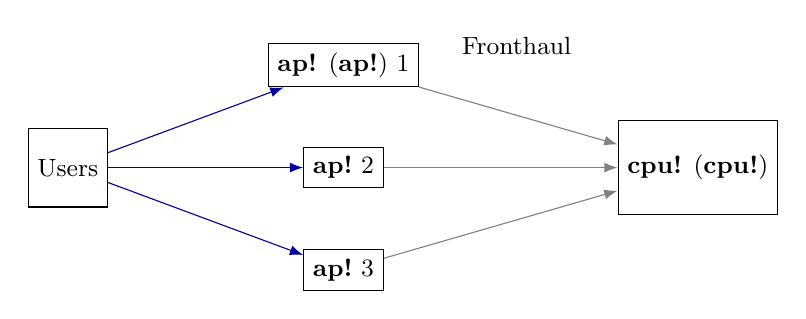
\begin{tikzpicture}[>=Latex,font=\small]
		\node[draw,minimum height=10mm](u)at(0,0){Users};
		\node[draw,minimum height=12mm](c)at(8,0){\ac{cpu}};
		\foreach \q/\y in {1/1.3,2/0,3/-1.3}{
			\node[draw](a\q)at(3.5,\y){\ac{ap} $\q$};
			\draw[->,blue!60!black](u)--(a\q);
			\draw[->,gray](a\q)--(c);
		}
		\node at(5.7,1.55){Fronthaul};
	\end{tikzpicture}
	\caption{Distributed \ac{ul} reception. Fronthaul exchanges received observations and relevant \ac{csi} for fully centralized processing, or locally processed outputs and supporting information for distributed processing and central fusion.}
	\label{fig06:distributed}
\end{figure}

\paragraph{Centralized and local combining.}
With fully centralized combining, the \ac{cpu} accesses the aggregate received observations and relevant \ac{csi} to construct a global combining matrix. This permits application of the centralized \ac{mimo} processing methods to the stacked channel.

With local combining, each \ac{ap} instead computes
\begin{equation*}
	r_{q,u}=\mH{\ma{w}}_{q,u}\ma{y}_q,
	\qquad
	\ma{w}_{q,u}\in\compl^{N_{\mathsf r,q}\times1},
\end{equation*}
and forwards the processed output to the \ac{cpu}, which forms
\begin{equation*}
	\widehat x_u=\sum_{q=1}^{Q}a_{q,u}^*r_{q,u}.
\end{equation*}
These operations can be represented by an aggregate combiner, but the feasible combining weights depend on the information available to the local processors and the \ac{cpu}. Mathematical partitioning of a centralized model does not inherently reduce performance; practical limitations arise from restricted observations, \ac{csi}, processing, fronthaul, quantization, delay, and synchronization.

\paragraph{Propagation and deployment effects.}
Distribution also changes the underlying channel statistics. Closer \acp{ap} may provide stronger channels to individual users, and spatially separated access points can reduce overlap between different user channels. However, received energy may become concentrated on relatively few dominant ports, weakening channel hardening. Improved user separation and stronger channel hardening are therefore not necessarily simultaneous benefits, and neither statistic alone determines the achievable rate.

\paragraph{Distributed \ac{dl} constraints.}
The aggregate \ac{dl} model remains applicable, but local precoders must satisfy individual \ac{ap} energy constraints,
\begin{equation*}
	\Ed\frob{\ma{F}_q}^2\leq E_q^{\mathsf{max}},
	\qquad
	\ma{F}_q\in\compl^{N_{\mathsf t,q}\times U}.
\end{equation*}
Coherent transmission requires suitable \ac{csi}, timing and phase coordination, and distribution of user data to participating \acp{ap}. User-centric serving sets $\set Q_u\subseteq\{1,\ldots,Q\}$ can limit which \acp{ap} participate in serving user $u$, reducing information exchange and computation at the cost of restricting cooperation.

\subsection{Comparison of representative \ac{mimo} configurations}
The principal digital \ac{mimo} configurations differ in message ownership, available processing cooperation, and energy and information constraints. Table~\ref{tab06:architectures} summarizes these distinctions.
\begin{longtable}{L{23mm}L{47mm}L{76mm}}
	\caption{Representative digital \ac{mimo} configurations and system constraints.}
	\label{tab06:architectures}\\
	\toprule
	Configuration & Ownership and processing & Constraints and objectives\\
	\midrule
	\endfirsthead
	\toprule
	Configuration & Ownership and processing & Constraints and objectives\\
	\midrule
	\endhead
	\ac{p2p} \ac{mimo}
	& One communication link with jointly processed streams; \ac{svd} or joint/linear reception
	& Common link-energy constraint; \ac{csir} and possibly \ac{csit}; spatial multiplexing, capacity, and reliability\\
	
	Conventional \ac{mu}-\ac{mimo}
	& Independent user messages; joint \ac{bs} reception in \ac{ul}, independent user receivers in \ac{dl}
	& Individual \ac{ul} energies; shared \ac{dl} energy; interference suppression, achievable rates, and fairness\\
	
	Massive \ac{mu}-\ac{mimo}
	& Same multiuser principles with many \ac{bs} ports and potentially many simultaneously served users
	& Spatial loading, favorable propagation, hardening, pilot overhead, hardware complexity, and energy efficiency\\
	
	Distributed \ac{mimo}
	& Spatially separated \acp{ap}; centralized or local processing with cooperation and fusion
	& Fronthaul, distributed \ac{csi}, synchronization, per-\ac{ap} energy limits, coverage, and user-centric cooperation\\
	\bottomrule
\end{longtable}

These configurations cannot be ranked independently of the comparison assumptions. Meaningful performance evaluations require consistent accounting of channel conditions, transmit energy, bandwidth, receiver cooperation, \ac{csi}, and implementation costs.

In \ac{tdd}, reciprocal propagation can support acquisition of \ac{dl} channel information through \ac{ul} training, provided the frontend responses are suitably calibrated and the channel remains coherent. In \ac{fdd}, separate \ac{dl} acquisition and feedback are generally necessary. Increasing the physical port count does not eliminate these acquisition requirements.

\subsection{Connecting the digital model to physical antenna arrays}
The previous lectures treated the effective digital channel as given. The complete \ac{mimo} system also includes physical antenna elements, \ac{rf} chains, and analog and digital frontend transformations. Using the established notation, the channel mappings are
\begin{equation}
	\boxed{
		\Hrf=\mH{\WA}\Ha\FA,
		\qquad
		\ma{H}=\mH{\WD}\Hrf\FD.
	}
	\label{eq06:frontend}
\end{equation}
The physical antenna channel is $\Ha\in\compl^{\NRa\times\NTa}$, the channel after analog processing is $\Hrf\in\compl^{\NRrf\times\NTrf}$, and the effective digital channel is $\ma{H}\in\compl^{\NR\times\NT}$. The corresponding frontend mappings have dimensions
\begin{equation*}
	\begin{aligned}
		\FA&\in\compl^{\NTa\times\NTrf},
		&\WA&\in\compl^{\NRa\times\NRrf},\\
		\FD&\in\compl^{\NTrf\times\NT},
		&\WD&\in\compl^{\NRrf\times\NR}.
	\end{aligned}
\end{equation*}
The stream precoder $\ma{F}$ and combiner $\ma{W}$ operate on the resulting digital signal ports. The system-interface definitions must avoid counting the same digital processing twice, and frontend transformations may produce nonwhite effective noise.

Part~II examines the physical origin of the channel coefficients and spatial structure used throughout Part~I. Lecture~07 begins with antenna positions, geometry, and spatial phase differences. Subsequent lectures develop array responses, beamforming architectures, antenna characteristics, and propagation-based \ac{mimo} channel models. These models explain how physical antenna and propagation configurations determine the effective digital-channel rank, singular values, correlation, and available spatial processing directions.


% ============================================================

% ============================================================
\clearpage
\section*{Summary and transition}
\addcontentsline{toc}{section}{Summary and transition}

The integrated examples consolidate the principal results of digital \ac{mimo} communications:

\begin{itemize}
	\item \textbf{Channel characterization:} Channel rank, singular values, conditioning, and spatial statistics determine the available spatial dimensions and their usefulness for transmission.
	
	\item \textbf{\ac{p2p} processing:} \ac{svd}-based precoding and combining separate spatial eigenchannels, while energy allocation determines how these modes are exploited to maximize achievable rate.
	
	\item \textbf{Multiuser processing:} \ac{mrc}/\ac{mrt}, \ac{zf}, and \ac{lmmse}/\ac{rzf} provide different tradeoffs between desired-signal gain, interuser interference, and noise or transmit-energy penalties.
	
	\item \textbf{\ac{csi} and detection:} Pilot-based estimation determines unknown channel coefficients, whereas data detection determines transmitted symbols using the available channel information. Estimation errors affect the performance of subsequent processing.
	
	\item \textbf{System performance:} Achievable rates and practical benefits depend on channel geometry, \ac{csi}, user loading, energy constraints, processing cooperation, and implementation architecture.
\end{itemize}

Part~I has examined digital \ac{mimo} processing for a given effective channel. Part~II investigates how physical antenna arrays, propagation geometry, antenna characteristics, and frontend architectures determine this channel and constrain the realizable spatial processing.

\end{document}


